\documentclass[a4paper,12pt]{article}
\usepackage{amsmath, bm}
\usepackage{amssymb,amsthm,graphicx}
\usepackage{enumitem}
\usepackage{color}
\usepackage{epsfig}
\usepackage{graphics}
\usepackage{pdfpages}
\usepackage{subcaption}
\usepackage[font=small]{caption}
\usepackage[hang,flushmargin]{footmisc} 
\usepackage{float}
\usepackage[figuresleft]{rotating}
\usepackage{tabularx}
\usepackage{booktabs}
\usepackage[mathscr]{euscript}
\usepackage{natbib}
\usepackage{setspace}
\usepackage{placeins}
\usepackage{ulem}
\usepackage[left=3cm,right=3cm,bottom=3cm,top=3cm]{geometry}
\numberwithin{equation}{section}
\allowdisplaybreaks[3]


% General

\newcommand{\reals}{\mathbb{R}}
\newcommand{\integers}{\mathbb{Z}}
\newcommand{\naturals}{\mathbb{N}}

\newcommand{\pr}{\mathbb{P}}        % probability
\newcommand{\ex}{\mathbb{E}}        % expectation
\newcommand{\var}{\textnormal{Var}} % variance
\newcommand{\cov}{\textnormal{Cov}} % covariance

\newcommand{\law}{\mathcal{L}} % law of X
\newcommand{\normal}{N}        % normal distribution 

\newcommand{\argmax}{\textnormal{argmax}}
\newcommand{\argmin}{\textnormal{argmin}}

\newcommand{\ind}{\mathbbm{1}} % indicator function
\newcommand{\kernel}{K} % kernel function
\newcommand{\wght}{W} % kernel weight
\newcommand{\thres}{\pi} % threshold parameter


% Convergence

\newcommand{\convd}{\stackrel{d}{\longrightarrow}}              % convergence in distribution
\newcommand{\convp}{\stackrel{P}{\longrightarrow}}              % convergence in probability
\newcommand{\convas}{\stackrel{\textrm{a.s.}}{\longrightarrow}} % convergence almost surely
\newcommand{\convw}{\rightsquigarrow}                           % weak convergence


% Theorem-like declarations

\theoremstyle{plain}

\newtheorem{theorem}{Theorem}[section]
\newtheorem{prop}[theorem]{Proposition}
\newtheorem{lemma}[theorem]{Lemma}
\newtheorem{corollary}[theorem]{Corollary}
\newtheorem*{theo}{Theorem}
\newtheorem{propA}{Proposition}[section]
\newtheorem{lemmaA}[propA]{Lemma}
\newtheorem{definition}{Definition}[section]
\newtheorem{remark}{Remark}[section]
\renewcommand{\thelemmaA}{A.\arabic{lemmaA}}
\renewcommand{\thepropA}{A.\arabic{propA}}
\newtheorem*{algo}{Clustering Algorithm}


% Theorem numbering to the left

\makeatletter
\newcommand{\lefteqno}{\let\veqno\@@leqno}
\makeatother


% Heading

\newcommand{\heading}[2]
{  \setcounter{page}{1}
   \begin{center}

   \phantom{Distance to upper boundary}
   \vspace{0.5cm}

   {\LARGE \textbf{#1}}
   \vspace{0.4cm}
 
   {\LARGE \textbf{#2}}
   \end{center}
}


% Authors

\newcommand{\authors}[4]
{  \parindent0pt
   \begin{center}
      \begin{minipage}[c][2cm][c]{5cm}
      \begin{center} 
      {\large #1} 
      \vspace{0.05cm}
      
      #2 
      \end{center}
      \end{minipage}
      \begin{minipage}[c][2cm][c]{5cm}
      \begin{center} 
      {\large #3}
      \vspace{0.05cm}

      #4 
      \end{center}
      \end{minipage}
   \end{center}
}

%\newcommand{\authors}[2]
%{  \parindent0pt
%   \begin{center}
%   {\large #1} 
%   \vspace{0.1cm}
%      
%   #2 
%   \end{center}  
%}


% Version

\newcommand{\version}[1]
{  \begin{center}
   {\large #1}
   \end{center}
   \vspace{3pt}
} 










\begin{document}



\heading{Clustering of epidemic time trends:}{the case of COVID-19}

%\authors{Marina Khismatullina\renewcommand{\thefootnote}{1}\footnotemark[1]}{University of Bonn}{Michael Vogt\renewcommand{\thefootnote}{2}\footnotemark[2]}{Ulm University} 
%\footnotetext[1]{Corresponding author. Address: Bonn Graduate School of Economics, University of Bonn, 53113 Bonn, Germany. Email: \texttt{marina.k@uni-bonn.de}.}
%\renewcommand{\thefootnote}{2}
%\footnotetext[2]{Address: Institute of Statistics, Department of Mathematics and Economics, Ulm University, 89081 Ulm, Germany. Email: \texttt{m.vogt@uni-ulm.de}.}
%\renewcommand{\thefootnote}{\arabic{footnote}}
%\setcounter{footnote}{2}

%\vspace{-0.85cm}

%\renewcommand{\baselinestretch}{1.2}\normalsize

%\renewcommand{\abstractname}{}
%\begin{abstract}
%\noindent The COVID-19 pandemic is one of the most pressing issues at present. A question which is particularly important for governments and policy makers is the following: Does the virus spread in the same way in different countries? Or are there significant differences in the development of the epidemic? In this paper, we devise new inference methods that allow to detect differences in the development of the COVID-19 epidemic across countries in a statistically rigorous way. In our empirical study, we use the methods to compare the outbreak patterns of the epidemic in a number of European countries.
%\end{abstract}

%\noindent \textbf{Key words:} simultaneous hypothesis testing; multiscale test; time trend; panel data; COVID-19.

%\noindent \textbf{JEL classifications:} C12; C23; C54.

%\noindent \textbf{AMS 2010 subject classifications:} 62E20; 62G10; 62G15; 62G20.

\renewcommand{\baselinestretch}{1.3}\normalsize



\section{Model}


Let $Y_{it}$ be the number of new COVID-19 infections on day $t$ in country $i$ and suppose we observe a time series $\mathcal{Y}_i = \{ Y_{it}: 1 \le t \le T \}$ for a large number $n$ of different countries $i$. In order to align the data of different countries, we take the starting date $t=1$ to be the first Monday after reaching $100$ confirmed cases in each country. Considering the dates after reaching a certain level of confirmed cases is a common practice of ``normalizing'' the data \citep[see e.g.][]{Cohen2020}. Starting on a Monday additionally aligns the data across countries by the day of the week. This allows us to take care of possible weekly cycles in the data which are produced by delays in reporting new cases over the weekend. 


We consider a simple nonparametric trend model for the time series $\mathcal{Y}_i$ in our sample. In particular, each time series $\mathcal{Y}_i$ is assumed to satisfy the nonparametric regression equation
\begin{equation}\label{eq:model}
Y_{it} = m_i\Big(\frac{t}{T}\Big) + u_{it} \qquad (1 \le t \le T) 
\end{equation}
with $\ex[u_{it}]= 0$, where $m_i$ is an unknown smooth trend curve defined on $[0,1]$. As usual in nonparametric regression \citep[see e.g.][]{Robinson1989}, we let the regression function $m_i$ in model \eqref{eq:model} depend on rescaled time $t/T$ rather than on real time $t$. The assumptions on the error term $u_{it}$ are discussed later. 


Even though the trend functions $m_i$ can be expected to be different across countries $i$, it is natural to assume that there are groups of countries $i$ with similar trend curves $m_i$. We thus impose a group structure on the countries in our sample. Informally speaking, we suppose that the countries can be grouped into a small number of classes such that within each class, all countries have the same trend function up to certain transformations. Formally speaking, the class structure is defined as follows: 
\begin{enumerate}[leftmargin=0.8cm]
\item[(G)] The set of countries $\{1,\ldots,n\}$ can be partitioned into $K$ groups $\mathcal{G}_1,\ldots,\mathcal{G}_K$ such that 
\[ m_i \in \class_k \quad \text{for all } i \in \mathcal{G}_k, \]
where $\mathcal{F}_k$ are function classes defined as
\[ \mathcal{F}_k := \big\{ f:[0, 1] \rightarrow \reals \,\big|\, f = c \cdot g_k(b \cdot u) \text{ with } c > 0, b \in [1, \bar{b}] \text{ and } g_k \text{ a density} \big\}. \]
The parameter $\bar{b}$ is assumed to be known. For identification purposes, the classes are supposed to be distinct, i.e., $\class_k \cap \class_{k^\prime} = \emptyset$ for any $k \neq k^\prime$. 
\end{enumerate}
As can be seen, the elements of the class $\mathcal{F}_k$ are rescaled versions of a density function $g_k$. Hence, all countries $i$ in the $k$-th group $\mathcal{G}_k$ have a trend curve $m_i$ that is a rescaled version of $g_k$, in particular, $m_i(u) = c \cdot g_k(b \cdot u)$ for some constants $c$ and $b$. We can regard $c$ as a country-specific scaling parameter that accounts for the size of the country or population density. We introduce this additional parameter in order to be able to compare countries with vastly different population sizes, e.g., Luxembourg and Russia. The constant $b$ can be interpreted as measuring the speed at which the epidemic develops in different countries. To see this, consider two countries $i$ and $j$ from the same group $k$ whose trend functions are given by $m_i(u) = g_k(b_i \cdot u)$ and $m_j(u) = g_k(b_j \cdot u)$ with $b_j > b_i$. (For simplicity, we set $c_i = c_j = 1$.) Obviously, we can write $m_j(u) = m_i(\{b_j/b_i\} u)$ for $u \in [0,b_i/b_j]$. Hence, the trend $m_j$ evolves qualitatively in the same way as $m_i$, but it evolves faster by the factor $b_j/b_i > 1$. 
%We can thus regard $b_j/b_i$ as measuring the relative speed of the development of the epidemic in country $j$ compared to $i$. 
In what follows, we call $b$ the effective time parameter of the model. 


\begin{remark}
The functions $m_i$ are not uniquely identified in terms of $c$, $b$ and $g_k$. In particular, we can rewrite $m_i(u) = c \cdot g_k(b \cdot u)$ as $m_i(u) = \tilde{c} \cdot \tilde{g}_k(u)$, where $\tilde{g}_k(u) = g_k(b \cdot u) / \int_{-\infty}^\infty g_k(b \cdot v) dv$ and $\tilde{c} = c \int_{-\infty}^\infty g_k(b \cdot v) dv$. To uniquely determine the quantities $c$, $b$ and $g_k$ in the definition of the classes $\mathcal{F}_k$, we additionally impose the following constraint: 
\begin{itemize}[leftmargin=0.75cm]
\item[(A)] For some $i_k \in \mathcal{G}_k$, it holds that $m_{i_k}(u) = c \cdot g_k(b \cdot u)$ with $b = 1$ and for all other $i \in \mathcal{G}_k$, $m_i(u) = c \cdot g_k(b \cdot u)$ with $b \ge 1$. 
\end{itemize}
Importantly, (A) is not an additional assumption but rather a harmless renormalization: If $m_i(u) = c \cdot g_k(b \cdot u)$ with $b > 1$ for all $i \in \mathcal{G}_k$, then we can replace $c$, $b$ and $g_k$ by renormalized versions $\tilde{c}$, $\tilde{b}$ and $\tilde{g}_k$ such that (A) holds. Also note that the classes $\mathcal{F}_k$ depend on the sample size $n$ in general (i.e., $\mathcal{F}_k = \mathcal{F}_{k,n}$) if we impose the normalization (A). For simplicity, however, we suppress the dependence on $n$ in the notation. 
\end{remark}


\pagebreak 
\begin{remark}
We could replace the above definition of $\mathcal{F}_k$ by the more general version 
\begin{align*}
\mathcal{F}_k := \big\{ f:[0, 1] \rightarrow \reals \,\big|\, & f = c \cdot g_k(b \cdot (u-u_0)) \text{ with } c>0, b \in [1, \bar{b}], \\ & u_0 \ge 0 \text{ and } g_k \text{ a density} \big\}. 
\end{align*}
However, since we have aligned the data across countries $i$ (by choosing the starting date $t=1$ to be the first Monday after reaching the $100$-th confirmed case in each country), we have implicitly normalized $u_0$ to be equal (to $0$) in each country. 
\end{remark}


Obviously, the group structure in the data is not observed. In particular, the groups $\mathcal{G}_1,\ldots,\mathcal{G}_K$, the group-specific density functions $g_1,\ldots,g_K$ and the number of groups $K$ are unknown in practice. In what follows, we construct a statistical procedure to estimate these quantities. 



\section{Clustering procedure}


In this section, we construct a hierarchical clustering algorithm to estimate the unknown group structure from the data. We first design a suitable dissimilarity measure and then build a HAC (Hierarchical Agglomerative Clustering) algorithm based on this measure.


\subsection{Construction of the dissimilarity measure} 


\begin{enumerate}[label=\textit{Step \arabic*.},leftmargin=1.45cm]


\item For each $i$, estimate $m_i(u)$ by a Nadaraya-Watson estimator with a rectangular kernel and bandwidth $h$, where we choose $h$ to be a multiple of $7$ days, i.e., $1$ week. This choice of bandwidth allows us to take care of possible weekly cycles in the data which are produced by delays in reporting new cases over the weekend. Formally, the estimator $\hat{m}_i(u)$ is defined as
\[ \hat{m}_i(u) =  \frac{ \sum_{t=1}^T K_h(u - \frac{t}{T}) Y_{it}}{\sum_{t=1}^T K_h(u - \frac{t}{T})} \]
with $K$ being a rectangular kernel and $K_h(x) = K(x/h)/h$. 


\item For a given value of $b \in [1, \bar{b}]$ and for a given pair of countries $(i, j)$, define the statistic
\[ \delta_{ij}(b) = \frac{1}{1/b} \int_0^{1/b} \bigg( \frac{\hat{m}_i (b\cdot u)}{\int_0^{1/b} \hat{m}_i(b\cdot v) dv /(1/b)}  - \frac{\hat{m}_j (u)}{\int_0^{1/b} \hat{m}_j(v) dv /(1/b)}  \bigg)^2 du. \]
This statistic measures a weighted $L_2$-distance between the functions $m_i(b \cdot u)$ and $m_j(u)$ on the interval $[0,1/b]$. Note that $\delta_{ij}(b) \neq \delta_{ji}(b)$ for $i \neq j$ in general.
%\textcolor{red}{(We should change the notation here: The argument $b$ of $\delta_{ij}$ does not play the same role as the parameter $b$ in the definition of $\mathcal{F}_k$.)}

%Suppose that countries $i$ and $j$ belong to the same class $\mathcal{G}_k$, i.e. $m_i(u) = c_i g_k (b_i u)$ and $m_j(u) = c_j g_k(b_j u)$. Without loss of generality, assume that $b_i \geq b_j$.  Since $Y_{it} = m_i(t/T) + u_{it}$, we can rewrite the estimators $\hat{m}_i$  as follows: 
%\begin{align*}
%\hat{m}_i(u) &= \sum_{t=1}^T \frac{K_h(u - t/T) (m_i(t/T) + u_{it})}{\sum_{s=1}^T K_h(u - s/T)} \\
%&= \sum_{t=1}^T \frac{K_h(u - t/T) (c_i g_k (b_i \cdot t/T) + u_{it})}{\sum_{s=1}^T K_h(u - s/T)}\\
%&=c_i  \sum_{t=1}^T \frac{K_h(u - t/T) g_k (b_i \cdot t/T)}{\sum_{s=1}^T K_h(u - s/T)} + \sum_{t=1}^T \frac{K_h(u - t/T) u_{it}}{\sum_{s=1}^T K_h(u - s/T)}
%\end{align*}

%Then for $b = b_i/b_j$ we have $m_i(u)/c_i = m_j(b u)/c_j$.


\item Aggregate the statistics $\delta_{ij}(b)$ for different values of $b$. Specifically, take the infimum over all possible values of $b$ to obtain the statistic
\[ \Delta_{ij} = \min \Big\{ \inf_{b\in [1, \bar{b}]} \delta_{ij}(b), \inf_{b\in [1, \bar{b}]} \delta_{ji}(b) \Big\}. \]


\item Let $S \subseteq \{1, \ldots, n\}$ and $S^\prime \subseteq \{1, \ldots, n\}$ be two sets of time series from our sample. There are several ways to define a dissimilarity measure between $S$ and $S^\prime$. We work with the complete linkage measure of dissimilarity defined as 
\begin{align*}
\mathcal{D} (S, S^\prime) = \max_{i \in S, j\in S^\prime} \Delta_{ij}.
\end{align*}
Alternatively, we may use a single or average linkage measure. 


\end{enumerate}


To understand the idea behind the statistic $\Delta_{ij}$ and thus the dissimilarity measure $\mathcal{D}$, let us suppose for a moment that we could perfectly estimate $m_i$ and $m_j$, that is, $\hat{m}_i = m_i$ and $\hat{m}_j = m_j$. For two countries $i$ and $j$ from the same group $\mathcal{G}_k$, it holds that $m_i(u) = c_i \cdot g_k(b_i \cdot u)$ and $m_j(u) = c_j \cdot g_k(b_j \cdot u)$ with some constants $b_i$, $b_j$, $c_i$, $c_j$ (where $b_j \ge b_i$ w.l.o.g.). Hence, the two terms in the definition of $\delta_{ij}(b)$ can be written as  
\begin{align*}
\frac{m_i (b\cdot u)}{\int_0^{1/b} m_i(b\cdot v) dv /(1/b)} & = \frac{g_k (b \cdot b_i \cdot u)}{\int_0^{1/b} g_k(b \cdot b_i \cdot v) dv /(1/b)} \\
\frac{m_j (u)}{\int_0^{1/b} m_j(v) dv /(1/b)} & = \frac{g_k (b_j \cdot u)}{\int_0^{1/b} g_k(b_j \cdot v) dv /(1/b)}.
\end{align*}
The two right-hand sides of the above display become identical upon setting $b = b_j/b_i$, which implies that $\delta_{ij}(b) = 0$. This suggests the following: $\delta_{ij}(b)$ tends to be small for some $b \in [1,\bar{b}]$ if $i$ and $j$ belong to the same group $\mathcal{G}_k$. Similar considerations suggest that $\delta_{ij}(b)$ tends to be large for all $b \in [1,\bar{b}]$ if $i$ and $j$ belong to different groups. As a consequence, we expect the statistic $\Delta_{ij}$ to be small/large if $i$ and $j$ belong to the same group/different groups. 


\subsection{HAC algorithm}\label{sec:alg}


The HAC algorithm based on the dissimilarity measure $\mathcal{D}$ proceeds as follows:
\begin{itemize}[leftmargin=1.4cm]

\item[\textit{Step 0}] \textit{(Initialization)}. Let $\hat{\mathcal{G}}_i^{[0]} = \{i\}$ denote the $i$th singleton cluster for $1 \leq i \leq n$ and define $\{\hat{\mathcal{G}}_1^{[0]}, \ldots, \hat{\mathcal{G}}_n^{[0]}\}$ to be the
initial partition of time series into clusters.

\item[\textit{Step r}] \textit{(Iteration)}. Let $\hat{\mathcal{G}}^{[r-1]}_1, \ldots, \hat{\mathcal{G}}^{[r-1]}_{n - (r-1)}$ be the $n-(r-1)$ clusters from the previous step. Determine the pair of clusters $\hat{\mathcal{G}}^{[r-1]}_k$ and $\hat{\mathcal{G}}^{[r-1]}_{k^\prime}$ for which 
\begin{align*}
\mathcal{D}(\hat{\mathcal{G}}^{[r-1]}_{k}, \hat{\mathcal{G}}^{[r-1]}_{k^\prime}) = \min_{1 \leq l < l^\prime \leq n- (r-1)} \mathcal{D}(\hat{\mathcal{G}}^{[r-1]}_{l}, \hat{\mathcal{G}}^{[r-1]}_{l^\prime})
\end{align*}
and merge them into a new cluster.

\end{itemize}
Iterating this procedure for $r = 1, \ldots, n-1$ yields a tree of nested partitions $\{\hat{\mathcal{G}}^{[r]}_1, \ldots, \hat{\mathcal{G}}^{[r]}_{n-r} \}$, which can be graphically represented by a dendrogram. Roughly speaking, the HAC algorithm merges the $n$ singleton clusters $\hat{\mathcal{G}}^{[0]}_i = \{i\}$ step by step until we end up with the cluster $\{1, \ldots, n\}$. In each step of the algorithm, the closest two clusters are merged, where the distance between clusters is measured in terms of the dissimilarity $\mathcal{D}$. % We refer the reader to \cite{Ward1963} for an early reference on HAC clustering and to Section 14.3.12 in \cite{HastieTibshiraniFriedman2009} for an overview of hierarchical clustering methods.

\vspace{10pt}


\noindent \textcolor{red}{@Oliver: \\
- We're not sure whether the construction in Section 2.1 gives a particularly good dissimilarity measure. We in particular wonder whether the statistics $\delta_{ij}(b)$ can be replaced by something else. E.g., one may use a version of $\delta_{ij}(b)$ with a different normalization than the integrals $\int_0^{1/b} \hat{m}_i(b\cdot v) dv /(1/b)$ and $\int_0^{1/b} \hat{m}_j(v) dv /(1/b)$. \\
- The procedure described in Sections 2.1 and 2.2 is essentially the idea from your notes (which are attached to this pdf). The main difference is that the constants $c$ and $b$ are not estimated. The constant $c$ ``drops out'' when considering the statistics $\delta_{ij}(b)$ and the constant $b$ is taken care of by minimizing over it. \\
- Directly estimating the constants seems to be difficult. Is it really possible to identify the constants as moments of the underlying density $g_k$ and thus to estimate them as mentioned in your notes? We ran into the following problem when trying to do so: Applying the substitution rule to the integrals $\int_0^1 u^\ell m_i(u) du$ produces integrals in terms of the density $g_k$. However, the integrals do in general not run over the whole support of $g_k$ (but only over some part of it which depends on the specific values of the constants $b$ and $a$ in your notes) ... Maybe, we've misunderstood something here. If the constants could indeed be identified and estimated in terms of the moments of the underlying densities, this would be much simpler and better. So it would be great if you could help with that. 
}



%\section{Forecasting} 


%\textcolor{red}{Maybe it is possible to use the clustering procedure for forecasting?! Consider the $k$-th group $\mathcal{G}_k$: Let $m_i(u) = c_i \cdot g_k(b_i \cdot u)$ for all $i \in \mathcal{G}_k$ and let $i_0$ be such that $b_{i_0} < b_i$ for all $i \in S \subset \mathcal{G}_k$. Then, one could construct a forecast of $m_{i_0}$ as follows: 
%\[ m_{i_0}(u) = \frac{1}{\# S} \sum_{i \in S} \frac{c_{i_0}}{c_i} \,  m_i\Big( \frac{b_{i_0}}{b_i} u \Big) \quad \text{for } u \in \Big[1,\underbrace{\min_{i \in S} \Big\{ \frac{b_i}{b_{i_0}} \Big\}}_{>1} \Big]. \]
%The idea is to use those trends $m_i$ in the group $\mathcal{G}_k$ that evolve more quickly than $m_{i_0}$ (in the sense that $b_{i_0} < b_i$) to predict the future development of $m_{i_0}$. (One drawback of this approach is that the forecast of $m_{i_0}$ will in general be discontinuous at the time point $u=1$ as we plug estimators into the above formula.)  
%}
%\vspace{10pt}


%\noindent \textcolor{red}{@Oliver: Do you think this is a good idea that we should pursue??? Not sure about that...} 



\section{Empirical analysis}\label{sec:app}


In Section \ref{subsec:sim}, we assess the finite sample performance of our clustering method by Monte-Carlo experiments. In Section \ref{subsec:app}, we apply the method to a sample of COVID-19 data from $104$ different countries.


\subsection{Simulation}\label{subsec:sim}


\textcolor{red}{Not done yet.} 


\subsection{Analysis of COVID-19 data}\label{subsec:app}


%\subsubsection{Data}


We analyze data from $104$ countries. We consider only those countries that have a total number of at least $20\,000$ cases of infection during the considered time period. For each country $i$, we observe a time series $\mathcal{Y}_i = \{ Y_{it}: 1 \le t \le T \}$, where $Y_{it}$ is the number of newly confirmed COVID-19 cases in country $i$ on day $t$. The data are freely available on the homepage of the European Center for Disease Prevention and Control (\texttt{https://www.ecdc.europa.eu}) and were downloaded on 25 February 2021.\footnote{ECDC switched to a weekly reporting schedule for the COVID-19 situation on 17 December 2020. Hence, all daily updates have been discontinued from 14 December. The downloaded daily data set thus presents historical data until 14 December 2020.} As already mentioned in the Introduction, we take the first Monday after reaching $100$ confirmed cases in each country as the starting date $t=1$. 
Beginning the time series of each country on the day when that country reached $100$ confirmed cases is a common way of ``normalizing'' the data \citep[see e.g.][]{Cohen2020}. Additionally aligning the data by Monday allows to take care of possible weekly cycles in the data which are produced by delays in reporting new cases over the weekend. 
The time series length $T$ is taken to be the longest interval for which we have observations for all $104$ countries. The resulting dataset thus consists of $n = 104$ time series, each with $T = 192$ observations. Some of the time series contain negative values which we replaced by $0$. Overall, this resulted in $14$ replacements.


We assume that the data $Y_{it}$ of each country $i$ in our sample follow the nonparametric trend model 
\[ Y_{it} = m_i\Big(\frac{t}{T}\Big) + u_{it} \]
from equation \eqref{eq:model} and we impose the group structure (G) on the data. 
%. As in the theoretical part of the paper, we assume that all of the countries $i$ can be partitioned into $K$ classes $\mathcal{G}_1, \ldots, \mathcal{G}_K$ such that for each $1 \leq k\leq K$ and for all $i \in \mathcal{G}_k$, $m_i(u) = c \cdot g_k(b \cdot u)$ for some $c>0$ and $b\in[1, \bar{b}]$. We thus suppose that the general shape of the time trends $m_i$ are the same (or at least very similar) in all countries $i$ in a given group $\mathcal{G}_k$, but the scale and time parameters may vary across countries from the same group. 
To implement the HAC algorithm, we make the following choices:
\begin{itemize}[leftmargin=0.6cm]
\item We take $\bar{b} = 2$ in the definition of the classes $\mathcal{F}_k$, which is more than sufficient for our purposes: As discussed above, $b$ is some sort of effective time parameter. Suppose that $m_j(u) = m_i(b \cdot u)$ for some $b > 1$ and all $u \in [0,1/b]$. In this case, the trend $m_j$ evolves more quickly than $m_i$ by the factor $b$. By setting $\bar{b} = 2$, we allow the trend $m_j$ of country $j$ to evolve at most twice as quickly as the trend $m_i$ of country $i$.  
%Throughout the section, we set implement the clustering procedure in exactly the same way as in the simulation study of Section \ref{subsec:sim}. In particular, 
\item We use a rectangular kernel $K$ to compute the Nadaraya-Watson smoothers $\hat{m}_{i}$ and consider the bandwidths $h = 3.5/T$ and $h = 7/T$, which corresponds to effective sample sizes of $7$ and $14$ days of data respectively. 
\item We assume that the number of classes $K$ is equal to $7$. \textcolor{red}{(We haven't considered the problem of estimating $K$ yet. So far, $K$ is handpicked. @Oliver: Any ideas how to estimate $K$???)}
\item The values $\delta_{ij}(b)$ and $\delta_{ji}(b)$ are calculated not for all $b\in [1, \bar{b}]$, but on a grid that consists of the values $\{1, 1.01, 1.02, \ldots, \bar{b}\}$. Since this grid is finite, we write $\min_{b \in [1, \bar{b}]} \delta_{ij}(b)$ and $\min_{b \in [1, \bar{b}]} \delta_{ji}(b)$ instead of $\inf_{b \in [1, \bar{b}]} \delta_{ij}(b)$ and $\inf_{b \in [1, \bar{b}]} \delta_{ji}(b)$ in what follows.
\end{itemize}


The estimation results for the bandwidth choice $h=3.5/T$ are presented in Figures \ref{fig:dend}--\ref{fig:map_14days}:
\begin{itemize}[leftmargin=0.6cm]
\item Figure \ref{fig:dend} shows the dendrogram of the HAC algorithm for $h = 3.5/T$. The different colours of the countries correspond to the different classes they belong to. 
\item Figures \ref{fig:cl1}--\ref{fig:cl7} depict the trend functions of the countries in the different estimated classes, each figure corresponding to a specific class. Since the functions $m_i$ in a given class $\mathcal{G}_k$ are only identical up to the scaling by the constants $c$ and $b$, we do not plot the (estimated) functions $m_i$ themselves. We rather proceed as follows: Consider a specific class $\mathcal{G}_k$,  write the trends in this class as $m_i(u) = c_i \cdot g_k(b_i \cdot u)$ with some constants $c_i$ and $b_i$, and fix some country $i_k \in \mathcal{G}_k$. It holds that $m_i(u) = \{ c_{i_k}/c_i \} \cdot m_i(\{ b_{i_k}/b_i \} u)$ for all $i \in \mathcal{G}_k$. Hence, the functions $\{ c_{i_k}/c_i \} \cdot m_i(\{ b_{i_k}/b_i \} u)$ are identical for all $i \in \mathcal{G}_k$. Rather than plotting the estimates $\hat{m}_i(u)$, we thus pick some $i_k \in \hat{\mathcal{G}}_k$ and plot the renormalized functions $\{ \hat{c}_{i_k}/\hat{c}_i \} \cdot \hat{m}_i(\{ \hat{b}_{i_k}/\hat{b}_i \} u)$, where $\hat{c}_{i_k}/\hat{c}_i$ and $\hat{b}_{i_k}/\hat{b}_i$ are estimates of the ratios $c_{i_k}/c_i$ and $b_{i_k}/b_i$. (The index $i_k$ is chosen such that $\hat{b}_{i_k}/\hat{b}_i < 1$ for all $i \in \hat{\mathcal{G}}_k$.) 
\item Figure \ref{fig:map} shows the estimated clusters in a world map. As in Figure \ref{fig:dend}, the different colours of the countries correspond to the different classes they belong to. 
\end{itemize}
Figures \ref{fig:dend_14days}--\ref{fig:map_14days} present the corresponding results for $h=7/T$. 




%For comparability reasons, we plot $\hat{m}_i(\hat{b}_i \cdot u) / \hat{c}_i$ instead of $\hat{m}_i(u)$, where $\hat{b}_i$ and $\hat{c}_i$ are computed according to \eqref{eq:b_hat} and \eqref{eq:c_hat} in the following algorithm:
%\begin{enumerate}[label=\textit{Step \arabic*.},leftmargin=1.45cm]


%\item Compute the following quantities:
%\begin{align*}
%b_{ij} &= \begin{cases}
%\arg \min_{b \in [1, \bar{b}]} \delta_{ij}(b)  &\text{ if } \min_{b \in [1, \bar{b}]} \delta_{ij}(b) \leq \min_{b \in [1, \bar{b}]} \delta_{ji}(b) \\
%1 &\text{ otherwise}
%\end{cases}\\
%b_{ji} &=\begin{cases}
%\arg \min_{b \in [1, \bar{b}]} \delta_{ji}(b)  &\text{ if } \min_{b \in [1, \bar{b}]} \delta_{ji}(b) < \min_{b \in [1, \bar{b}]} \delta_{ij}(b) \\
%1 &\text{ otherwise}.
%\end{cases}
%\end{align*}
%%The idea behind these values is that our algorithm estimates the dissimilarity measure between countries $i$ and $j$ to be the smallest when their respective time parameters are equal to $b_{ij}$ and $b_{ji}$. These quantities are calculated for all pairs $i$ and $j$ irrespective of countries $i$ and $j$ being in the same class. However, 
%If the countries $i$ and $j$ are in the same class $k$, we have that $m_i(u) = c_i \cdot g_k (b_i \cdot u)$ and $m_j(u) = c_j \cdot g_k( b_j \cdot u)$. Hence,
%$$m_i \Big( \frac{u}{b_i} \Big) / c_i= g_k (u) = m_j \Big( \frac{u}{b_j} \Big) /c_j,$$
%and thus,
%$$m_i (u) / c_i = m_j \Big( \frac{b_i}{b_j} u \Big) /c_j,$$
%or alternatively,
%$$m_i\Big( \frac{b_j}{b_i} u \Big) /c_i = m_j (u) / c_j.$$
%If $b_i \geq b_j$, then $b_{ji}$ can be regarded as an approximation of $b_i / b_j$ (and $b_{ij}$ should be equal to $1$), and if $b_i < b_j$, then $b_{ij}$ can be regarded as an approximation of $b_j/b_i$ (and $b_{ji}$ should be equal to $1$). In any case, $m_i( b_{ij} u ) /c_i \approx m_j (b_{ji} u) / c_j$.


%\item Using the quantities from Step 1, we pick a representative time series $i_k$ for each cluster $k$. If the cluster $k$ consists only of one element, then the representative time series is the only member of the cluster. If the number of elements is greater than $1$, the representative time series $i_k$ is the one with ``the fastest'' trend function, that is, 
%$$i_k = \arg \max_{i \in \hat{\mathcal{G}}_k} \# \{j \in \hat{\mathcal{G}}_k, \, j\neq i: b_{ij} = 1\}.$$
%The representative time series $i_k$ is plotted on the whole rescaled time interval $[0, 1]$, whereas all other time series $j \in \hat{\mathcal{G}}_k,\, j \neq i_k$ due to the smaller or equal time parameter (and thus slower speed of the development of the epidemic) are plotted on the (possibly smaller) time interval $\big[ 0, 1/\hat{b}_j \big]$. The representative time series in Figures \ref{fig:cl1}--\ref{fig:cl7} and \ref{fig:cl1_14days}--\ref{fig:cl7_14days} are shown in red, all of the other time series in the respective cluster are shown in black.


%\item The rule for determining the quantities $\hat{b}_j$ is as follows:
%\begin{align}\label{eq:b_hat}
%\hat{b}_{j} = \begin{cases}
%1, &\text{ if } j = i_k \text{ (representative country),}\\
%\min \Big\{1, \frac{b_{j i_{k}}}{b_{i_k j}}\Big\},  &\text{ otherwise.}
%\end{cases}
%\end{align}
%Note that by construction, $\hat{b}_j \geq 1$. Hence, $\big[ 0, 1/\hat{b}_j \big] \subseteq [0, 1]$ for all $j$.


%\item We finally calculate $\hat{c}_i$. As in the theoretical part of the paper, $\hat{c}_i$ can be regarded as a normalization parameter that accounts for the scale of the pandemic in country $i$:
%\begin{align}\label{eq:c_hat}
%\hat{c}_{i} = \frac{\int_0^{1/\hat{b}_i} \hat{m}_i(\hat{b}_i v) dv}{1/\hat{b}_i}.
%\end{align}


%\end{enumerate}


\newpage 
\FloatBarrier
\begin{sidewaysfigure}[t!]
%\begin{minipage}[t]{0.98\textwidth}
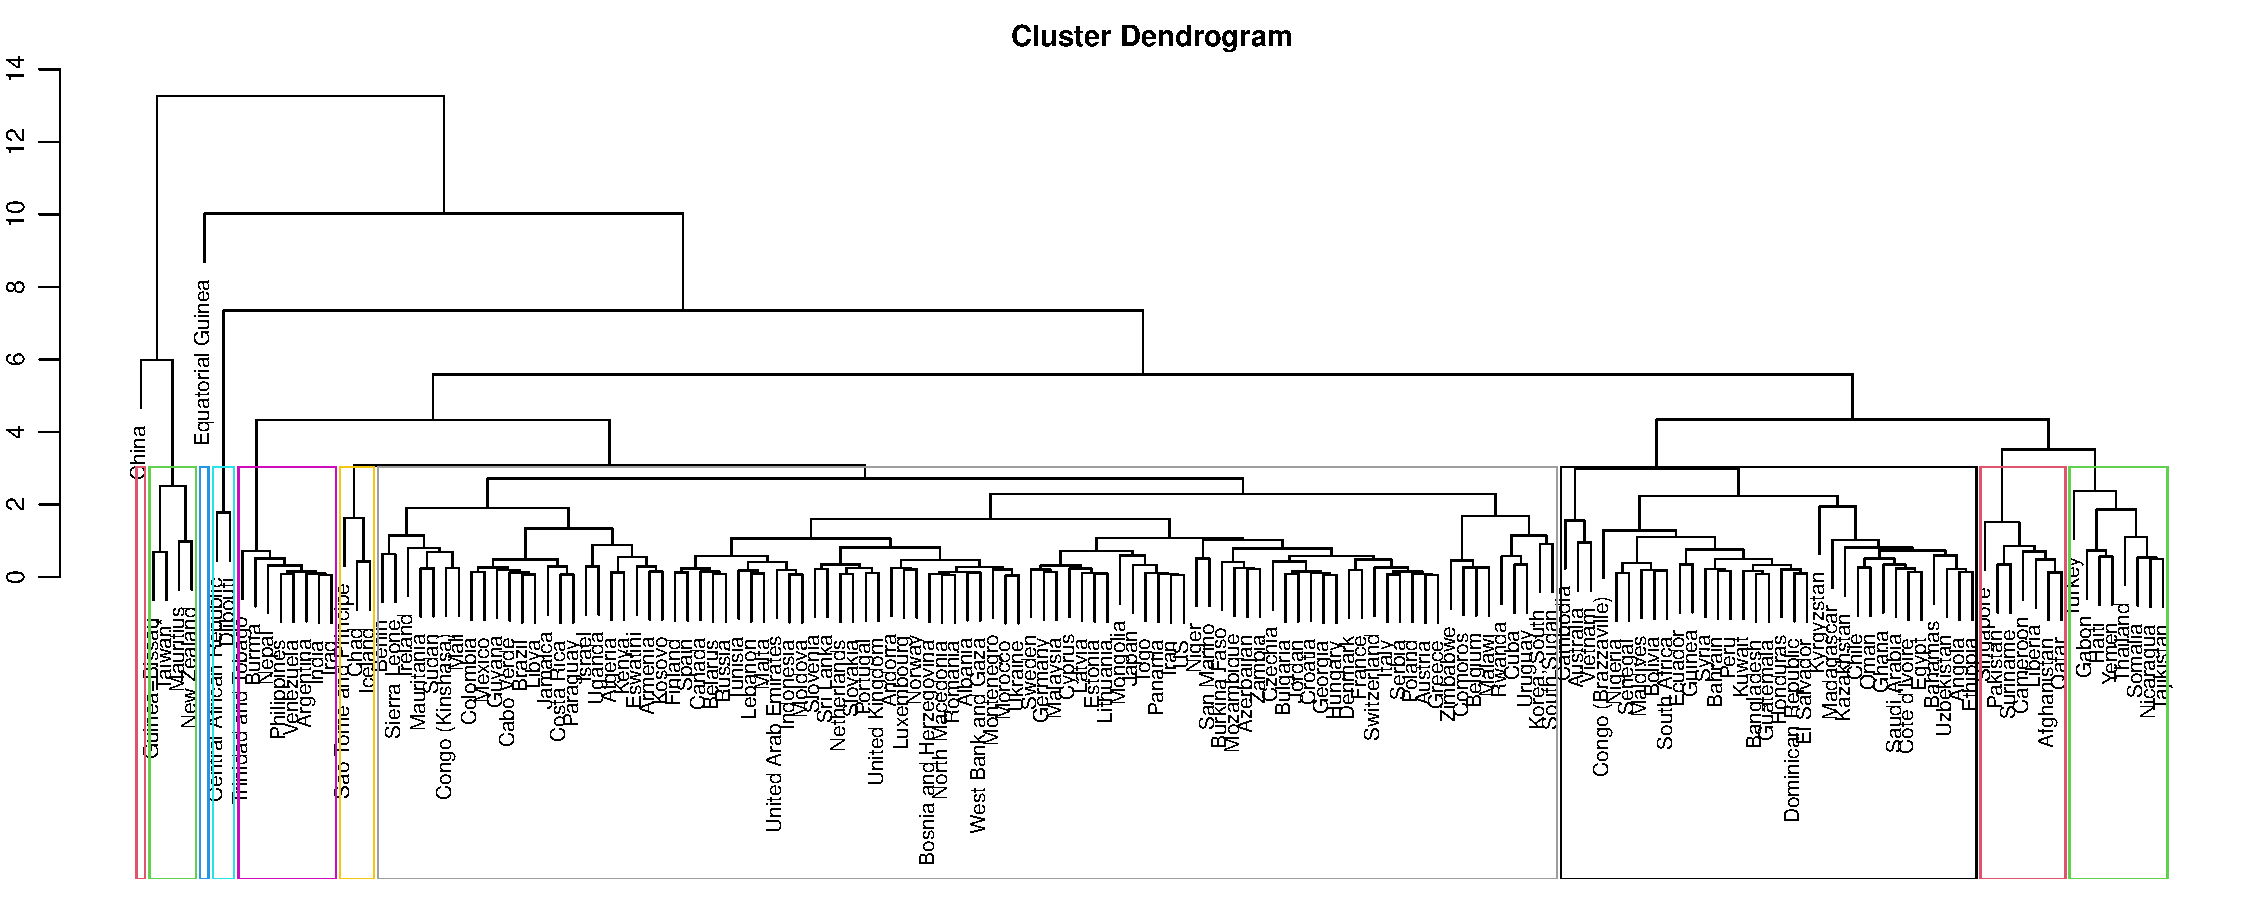
\includegraphics[width=\textwidth]{plots/dendrogram_10}
\caption{Results of HAC for $10$ clusters.}\label{fig:dend}
%\end{minipage}
\end{sidewaysfigure}

\newpage 
\FloatBarrier
\begin{sidewaysfigure}[t!]
%\begin{minipage}[t]{0.98\textwidth}
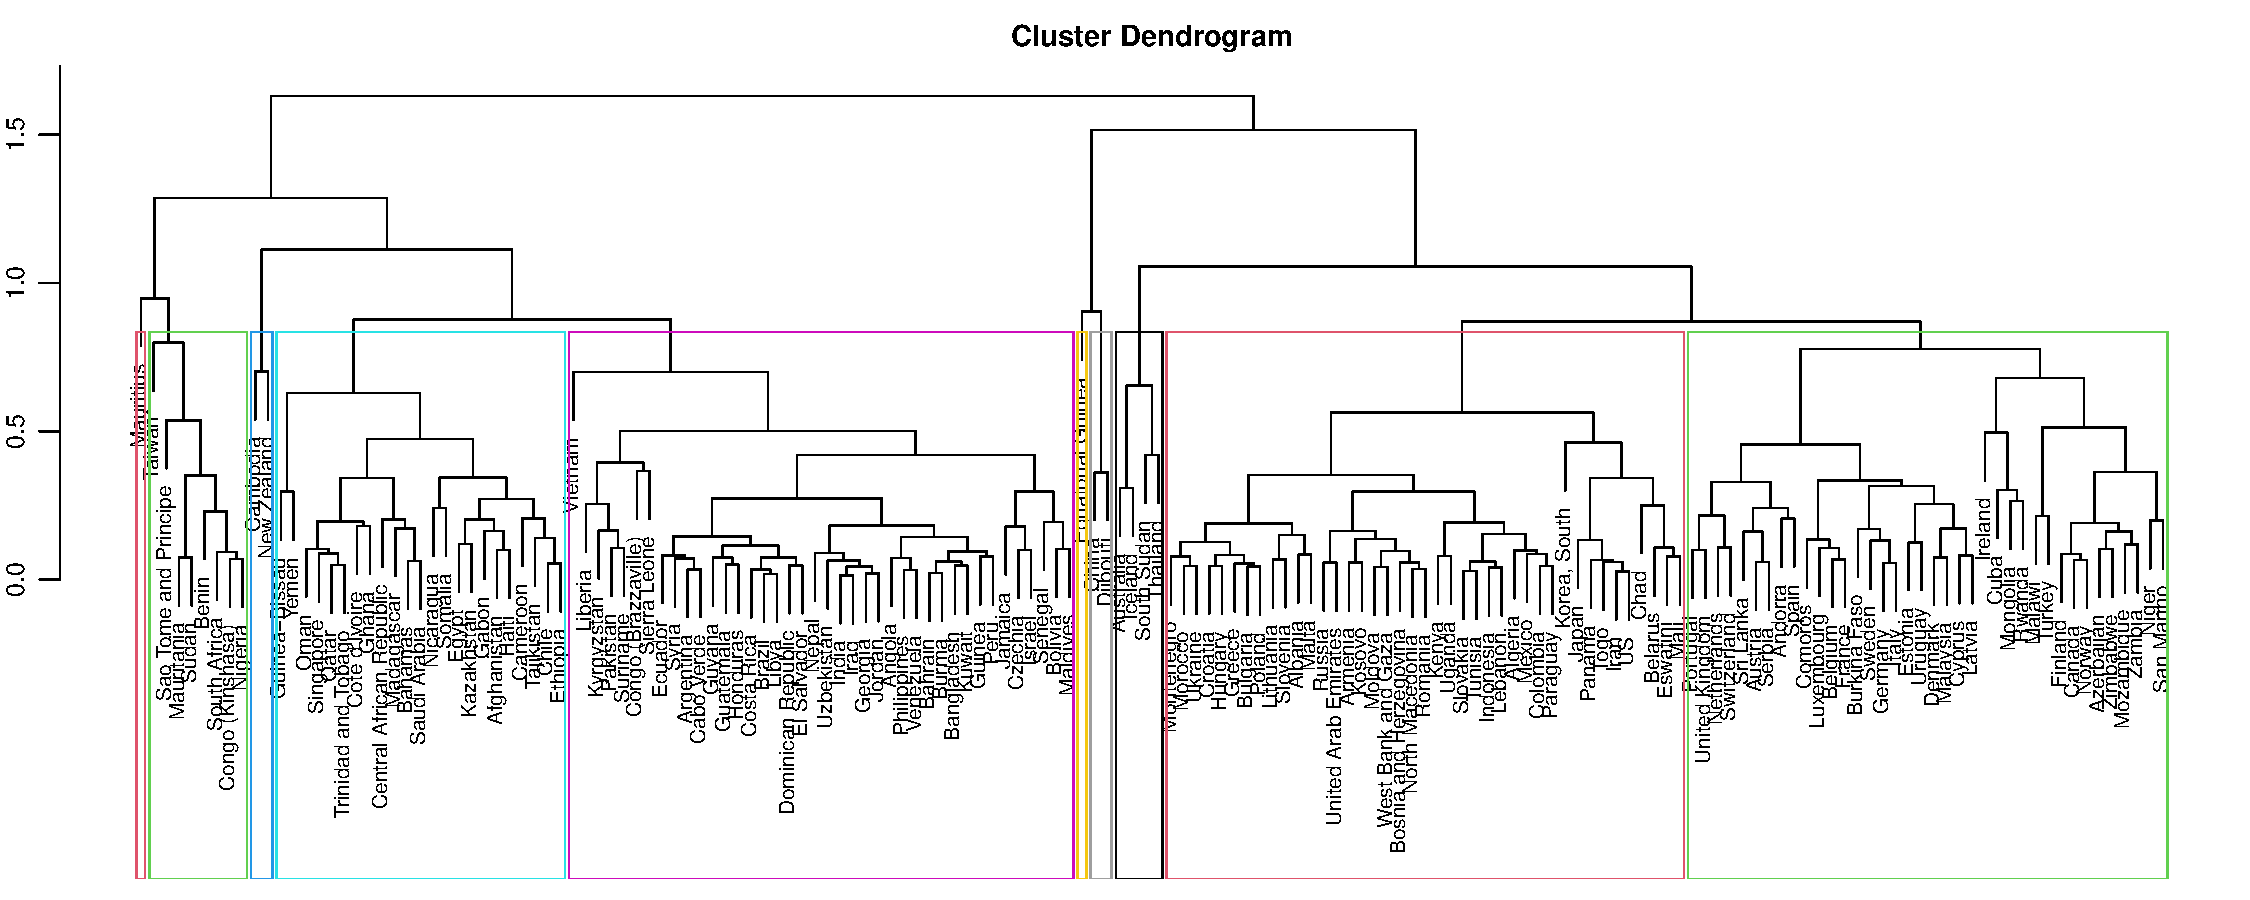
\includegraphics[width=\textwidth]{plots/dendrogram_alt_10}
\caption{Results of HAC for $10$ clusters, alternative approach}\label{fig:dend}
%\end{minipage}
\end{sidewaysfigure}


%\begin{figure}[t!]
%\centering
%\begin{subfigure}[b]{0.48\textwidth}
%\subfloat[][]{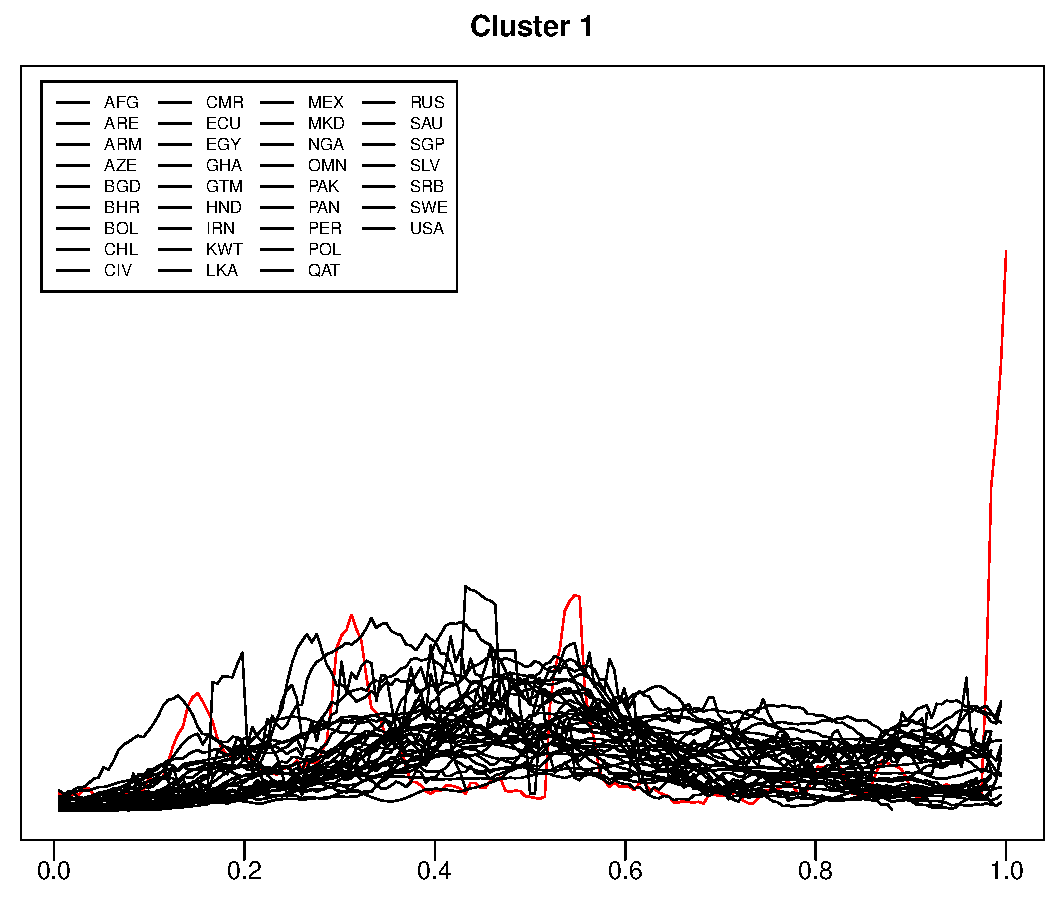
\includegraphics[width=\textwidth]{plots/7days/results_cluster_1}\label{fig:cl1}}
%\end{subfigure}\hspace{0.25cm}
%\begin{subfigure}[b]{0.48\textwidth}
%\subfloat[][]{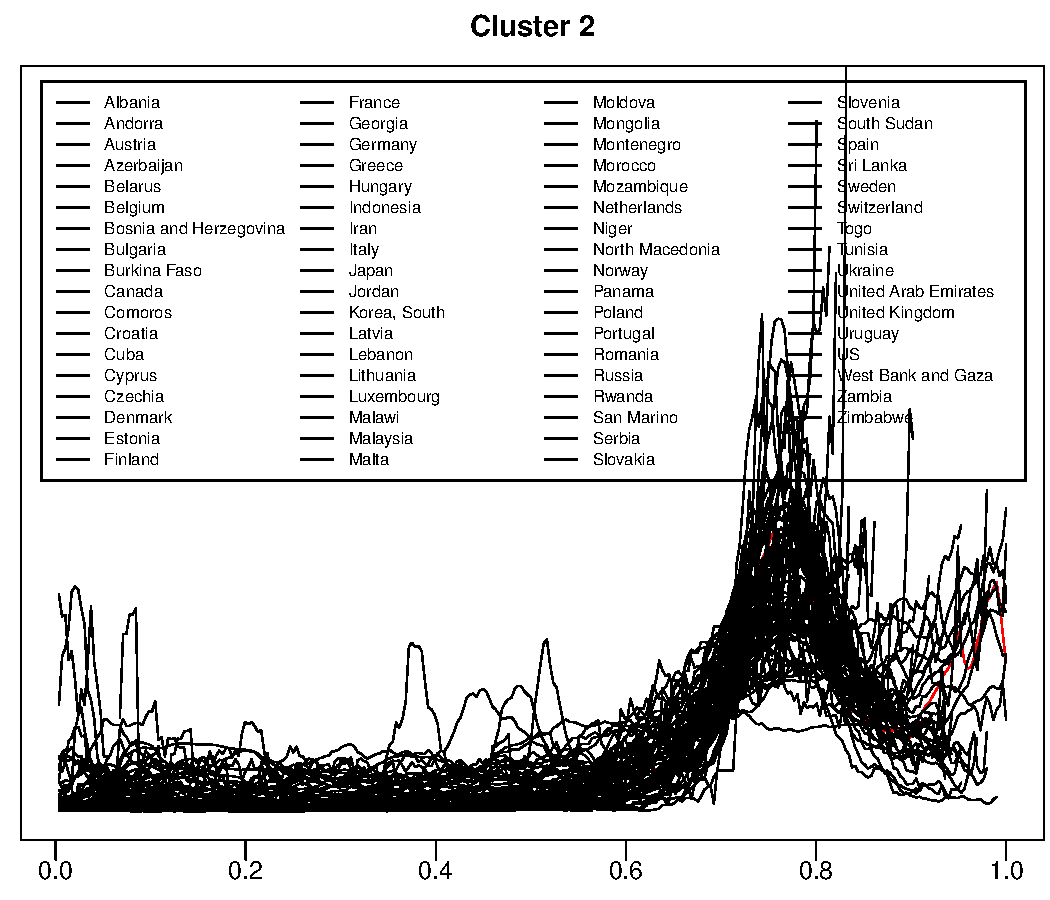
\includegraphics[width=\textwidth]{plots/7days/results_cluster_2}\label{fig:cl2}}
%\end{subfigure}\\
%\begin{subfigure}[b]{0.48\textwidth}
%\subfloat[][]{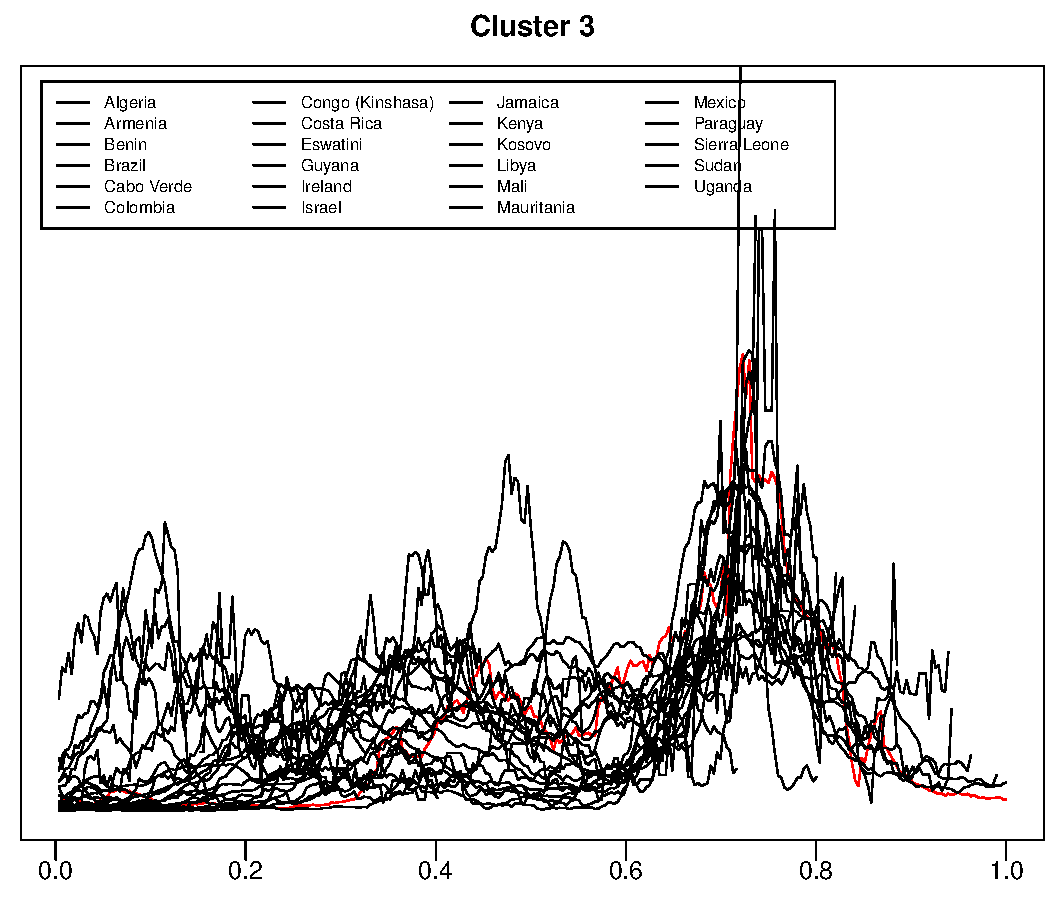
\includegraphics[width=\textwidth]{plots/7days/results_cluster_3}\label{fig:cl3}}
%\end{subfigure}\hspace{0.25cm}
%\begin{subfigure}[b]{0.48\textwidth}
%\subfloat[][]{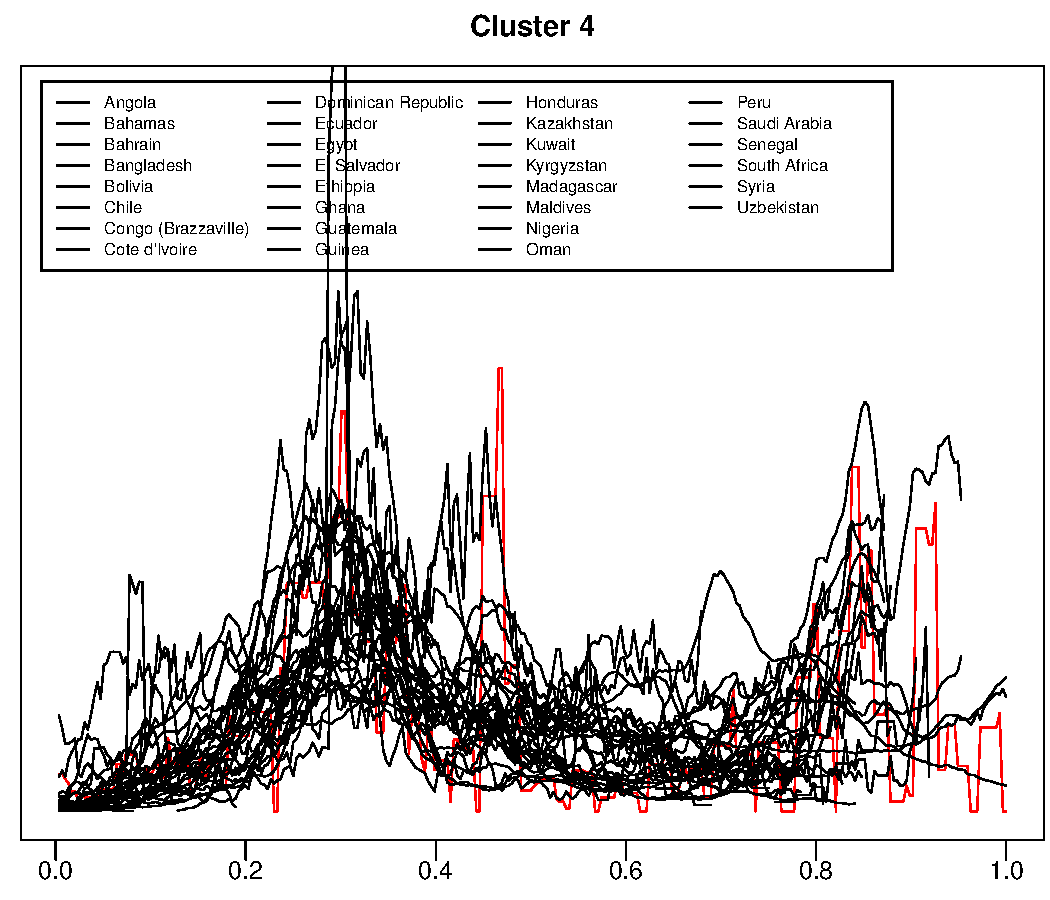
\includegraphics[width=\textwidth]{plots/7days/results_cluster_4}\label{fig:cl4}}
%\end{subfigure}\\
%\begin{subfigure}[b]{0.48\textwidth}
%\subfloat[][]{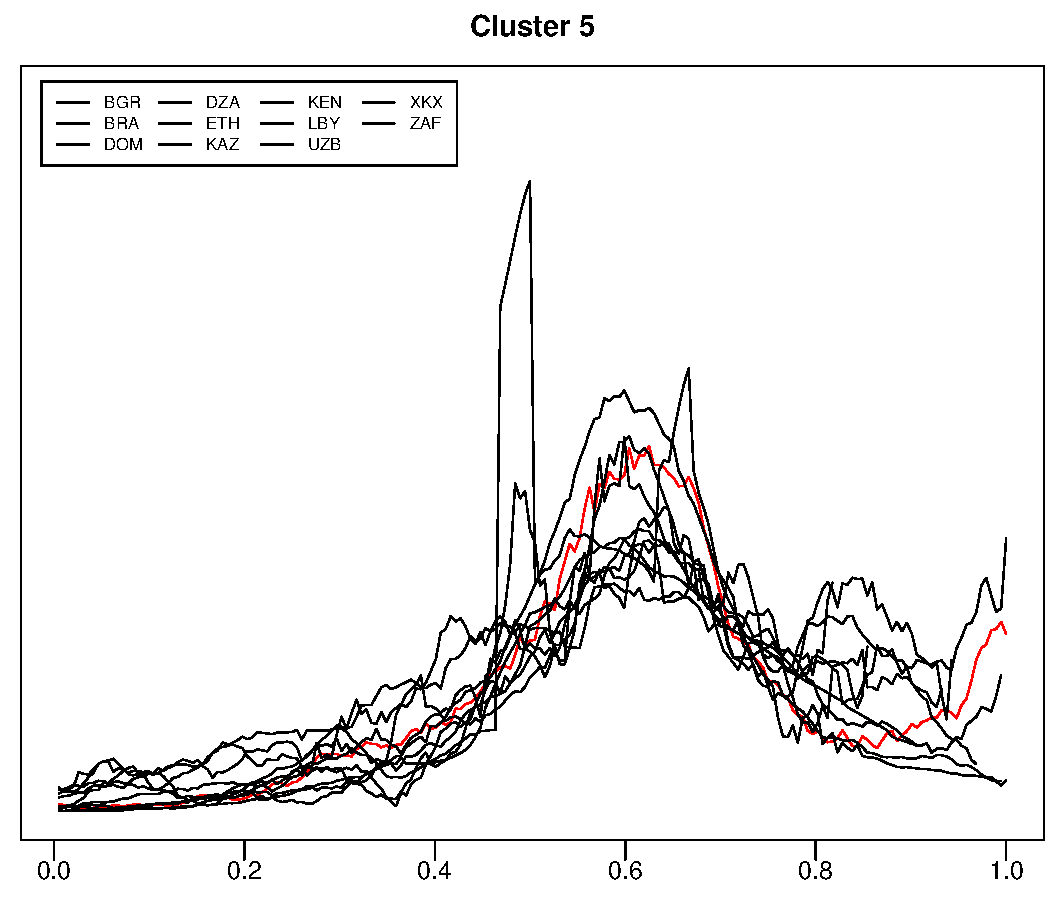
\includegraphics[width=\textwidth]{plots/7days/results_cluster_5}\label{fig:cl5}}
%\end{subfigure}\hspace{0.25cm}
%\begin{subfigure}[b]{0.48\textwidth}
%\subfloat[][]{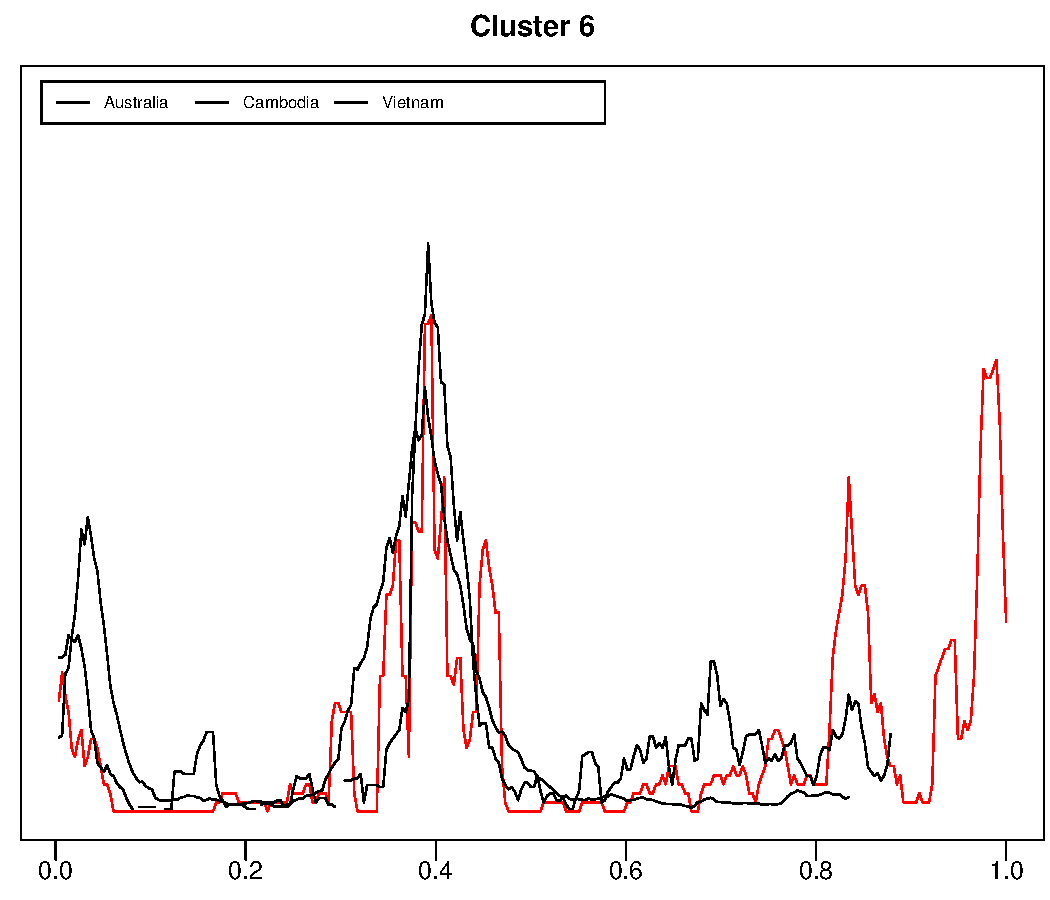
\includegraphics[width=\textwidth]{plots/7days/results_cluster_6}\label{fig:cl6}}
%\end{subfigure}
%\end{figure}
%
%\begin{figure}
%\ContinuedFloat
%\centering
%\begin{subfigure}[b]{0.48\textwidth}
%\subfloat[][]{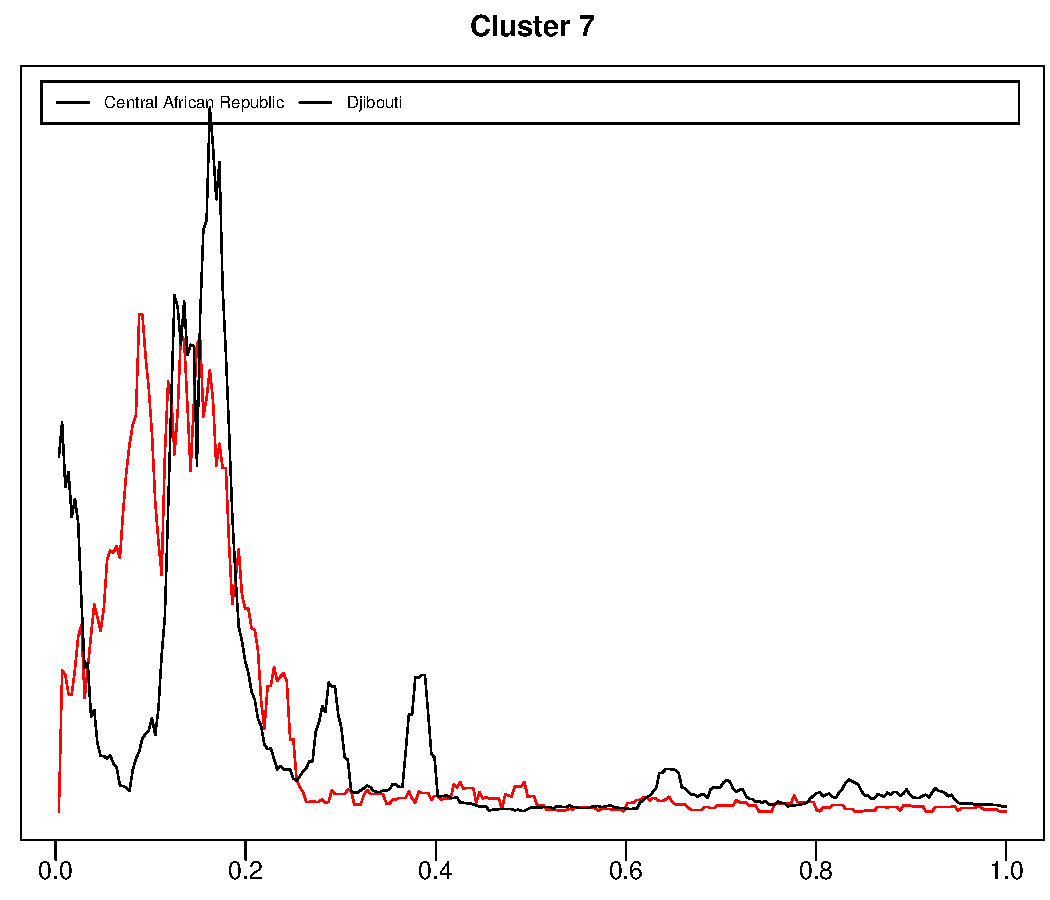
\includegraphics[width=\textwidth]{plots/7days/results_cluster_7}\label{fig:cl7}}
%\end{subfigure}
%\caption{Clusters produced by the algorithm. Each panel presents appropriately scaled curve estimates $\hat{m}_i$ that belong to a particular cluster. The bandwidth $h$ is taken to be $3.5/T$.}\label{fig:clusters}
%\end{figure}

\begin{figure}[t!]
\begin{minipage}[t]{0.98\textwidth}
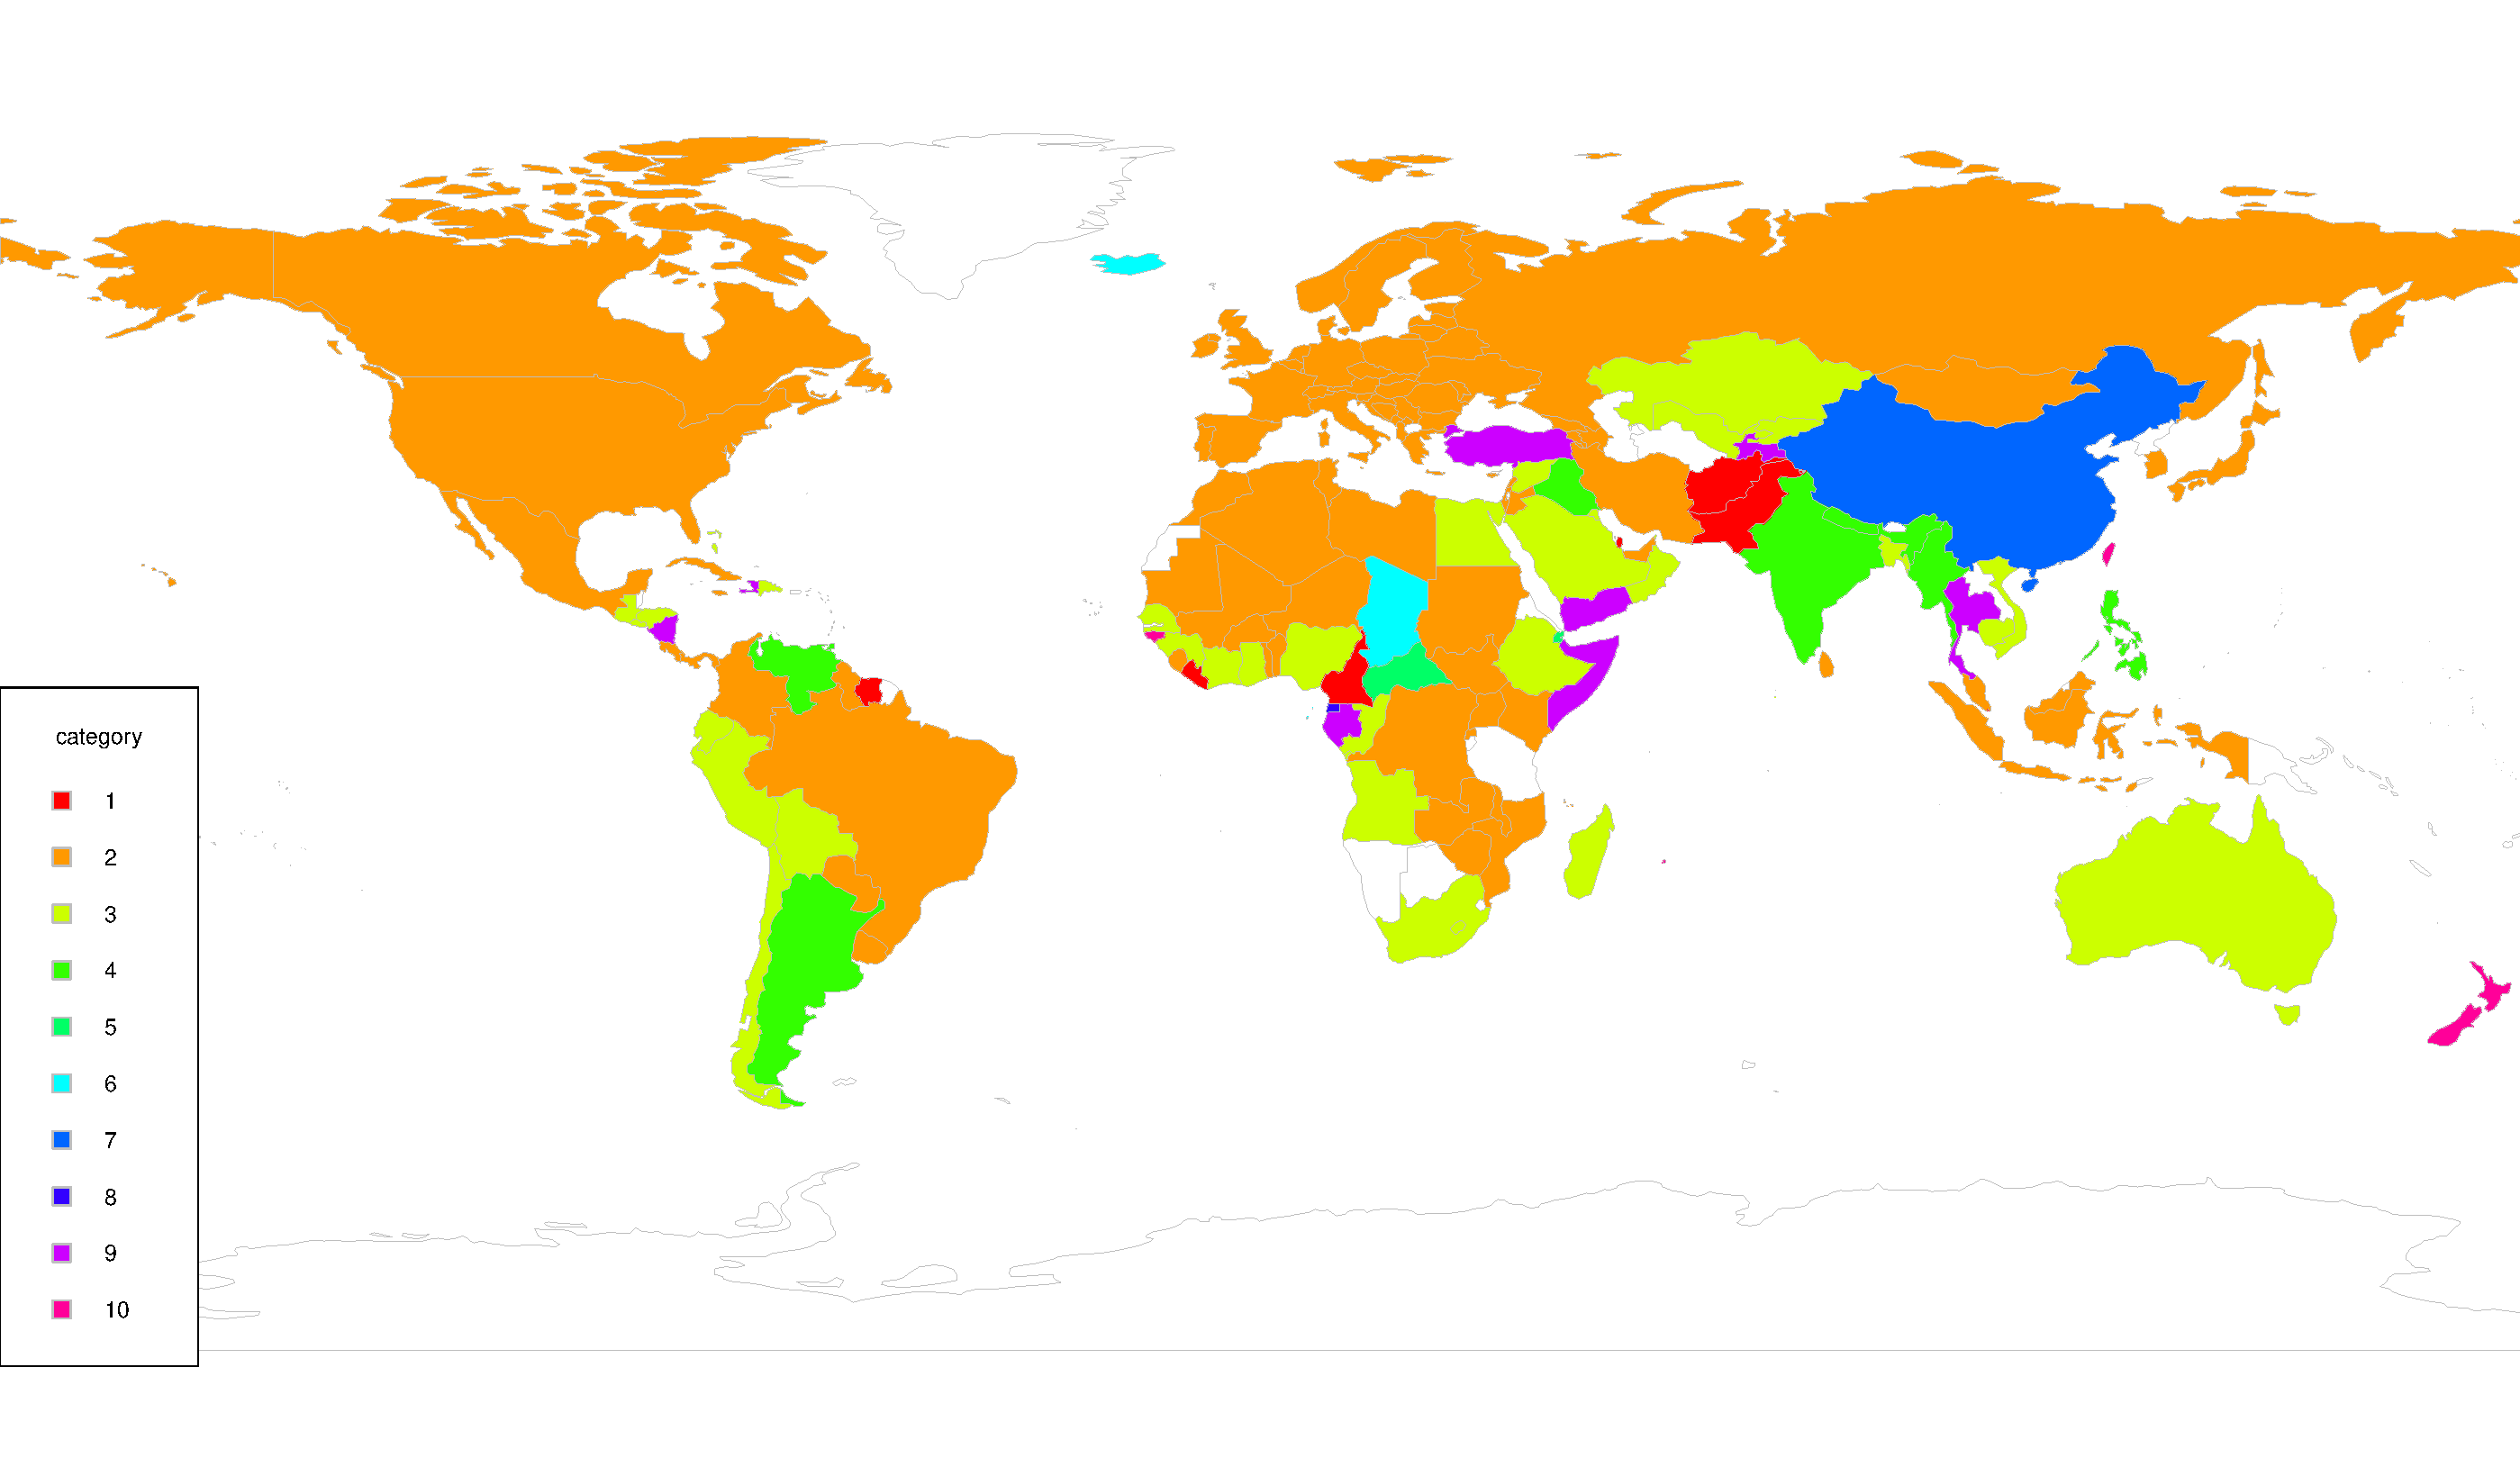
\includegraphics[width=\textwidth]{plots/choropleth_10}
\caption{Results of HAC for $10$ clusters on a map: each country is coloured according to the group it belongs to.}\label{fig:map}
\end{minipage}
\end{figure}

\begin{figure}[t!]
\begin{minipage}[t]{0.98\textwidth}
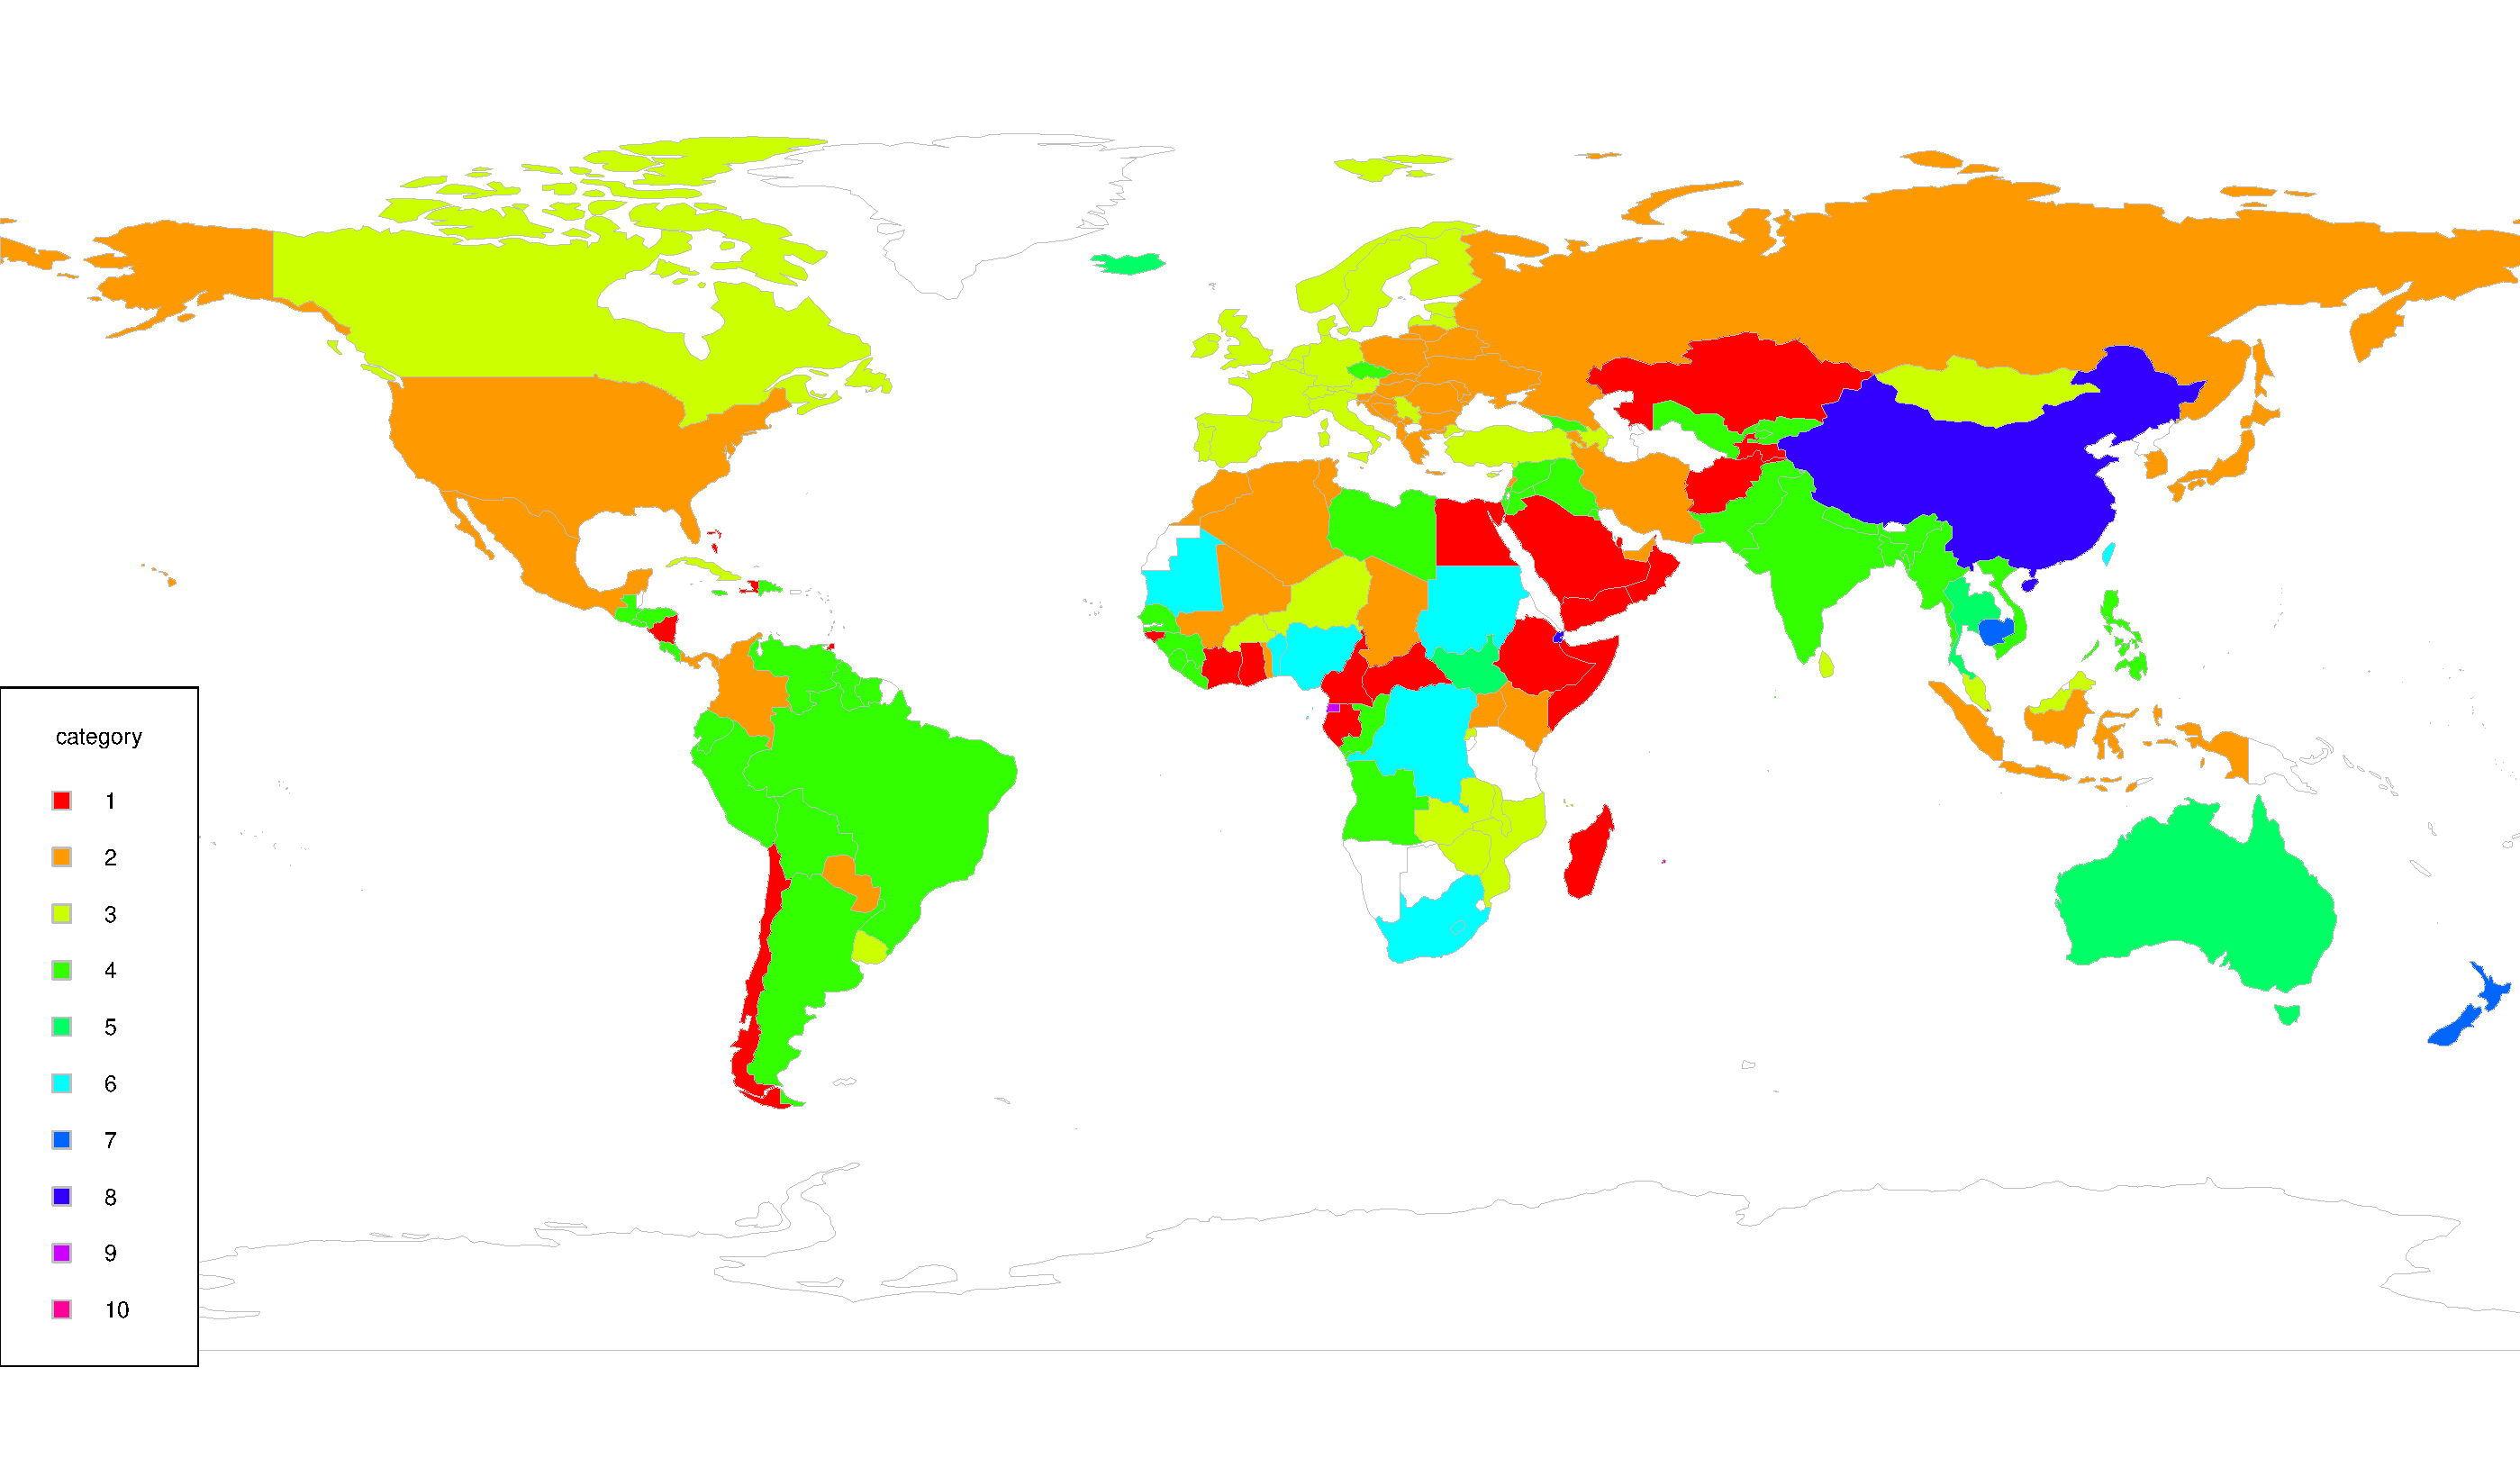
\includegraphics[width=\textwidth]{plots/choropleth_alt_10}
\caption{Results of HAC for $10$ clusters (alternative approach) on a map: each country is coloured according to the group it belongs to.}\label{fig:map}
\end{minipage}
\end{figure}


\newpage 
\FloatBarrier
\begin{sidewaysfigure}[t!]
%\begin{minipage}[t]{0.98\textwidth}
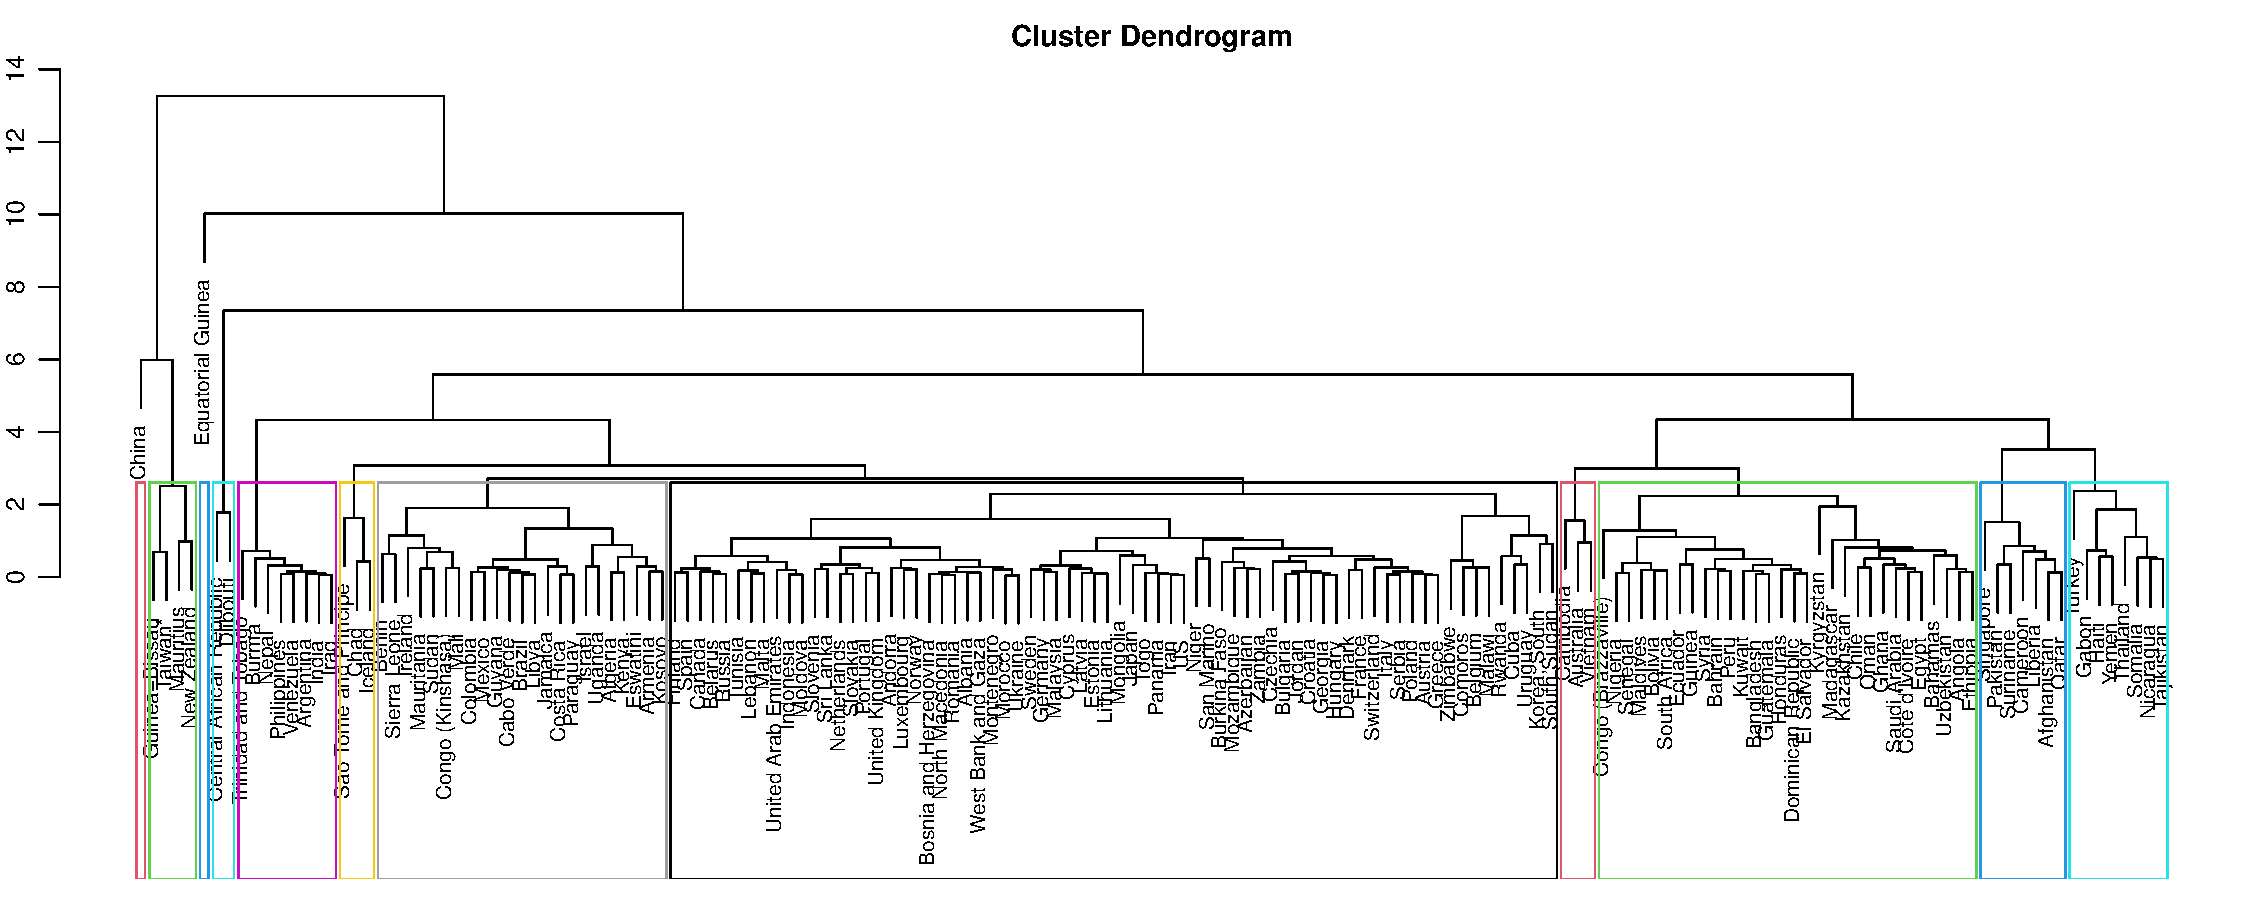
\includegraphics[width=\textwidth]{plots/dendrogram_12}
\caption{Results of HAC for $12$ clusters.}
%\end{minipage}
\end{sidewaysfigure}

\newpage 
\FloatBarrier
\begin{sidewaysfigure}[t!]
%\begin{minipage}[t]{0.98\textwidth}
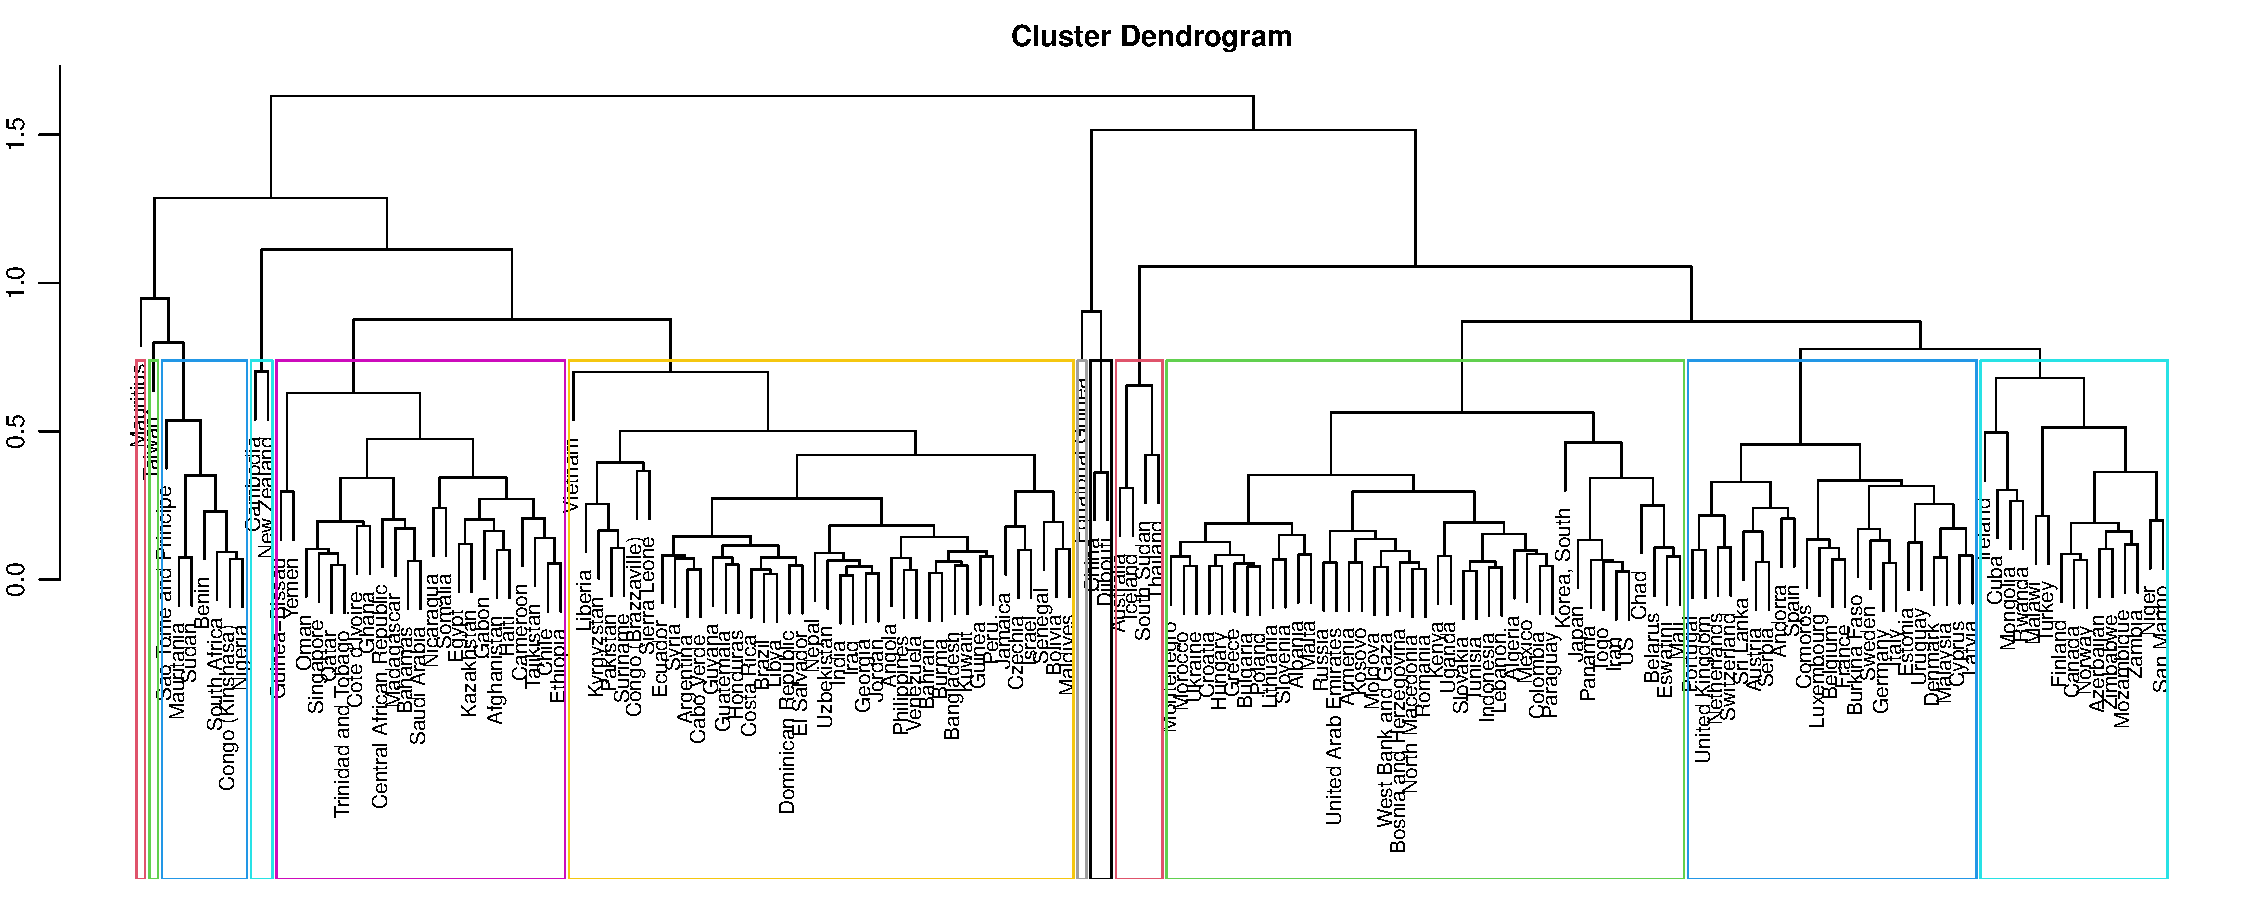
\includegraphics[width=\textwidth]{plots/dendrogram_alt_12}
\caption{Results of HAC for $12$ clusters, alternative approach}
%\end{minipage}
\end{sidewaysfigure}


\begin{figure}[t!]
\begin{minipage}[t]{0.98\textwidth}
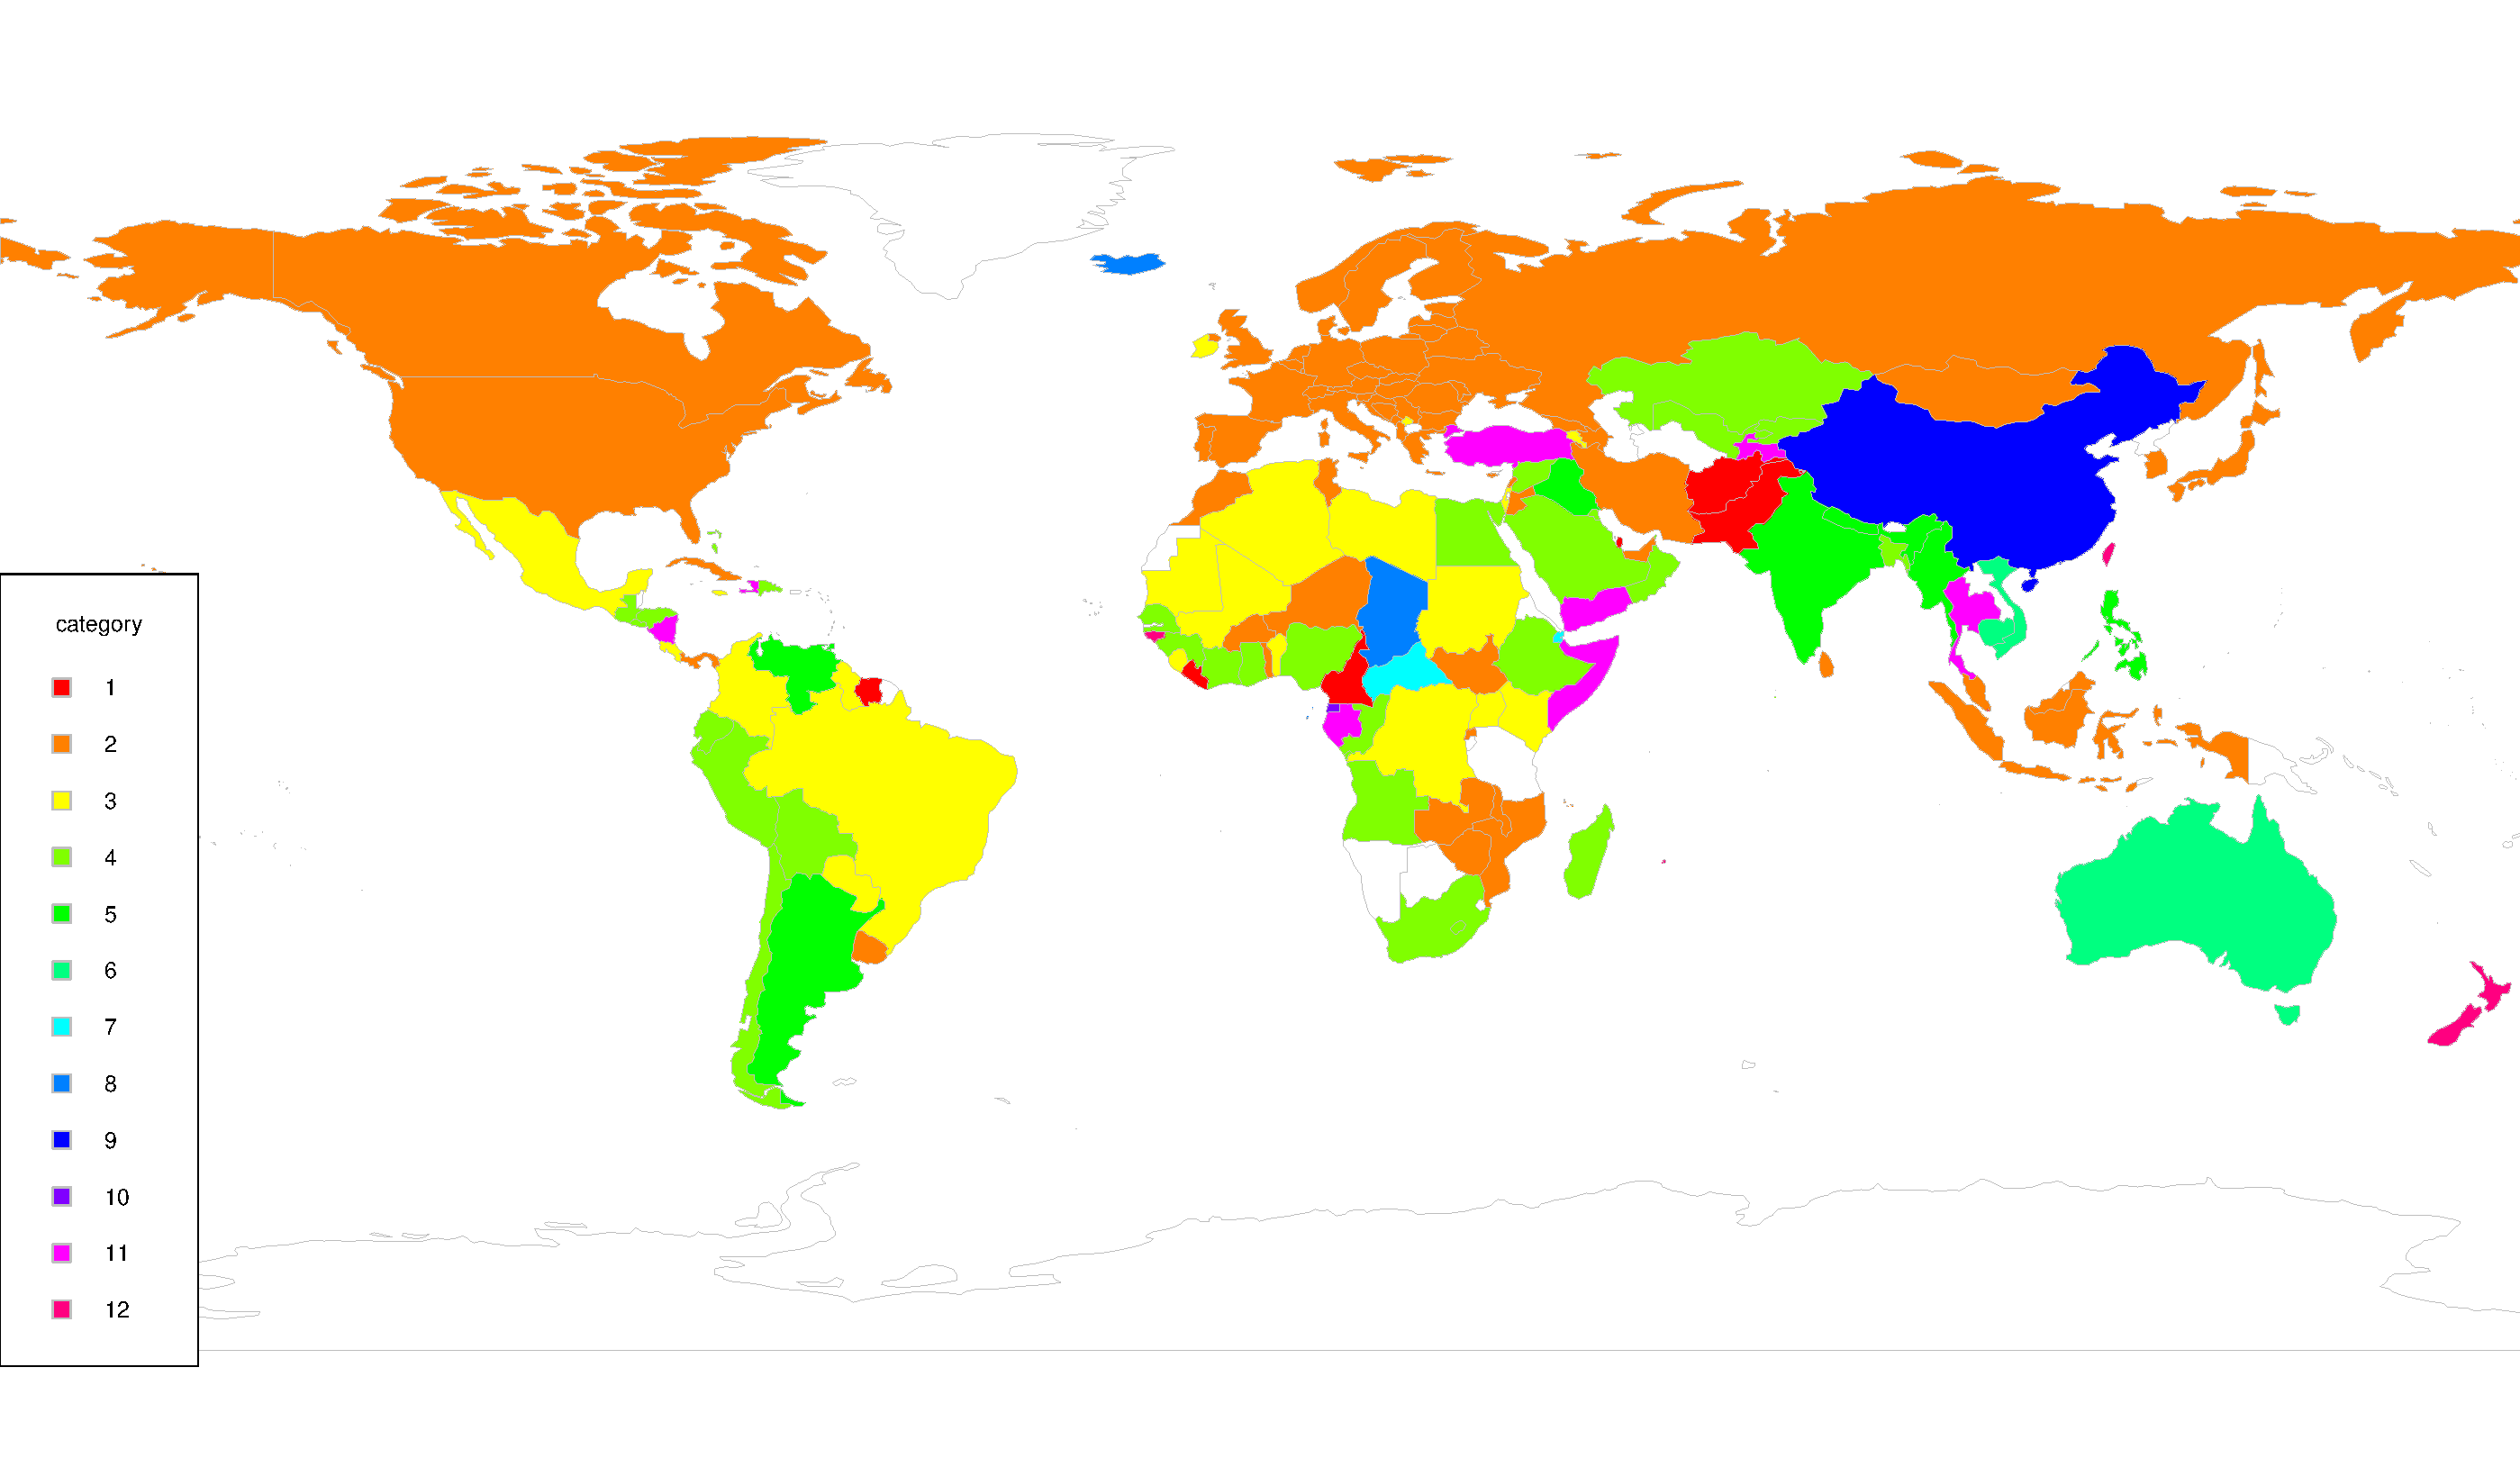
\includegraphics[width=\textwidth]{plots/choropleth_12}
\caption{Results of HAC for $12$ clusters on a map: each country is coloured according to the group it belongs to.}
\end{minipage}
\end{figure}

\begin{figure}[t!]
\begin{minipage}[t]{0.98\textwidth}
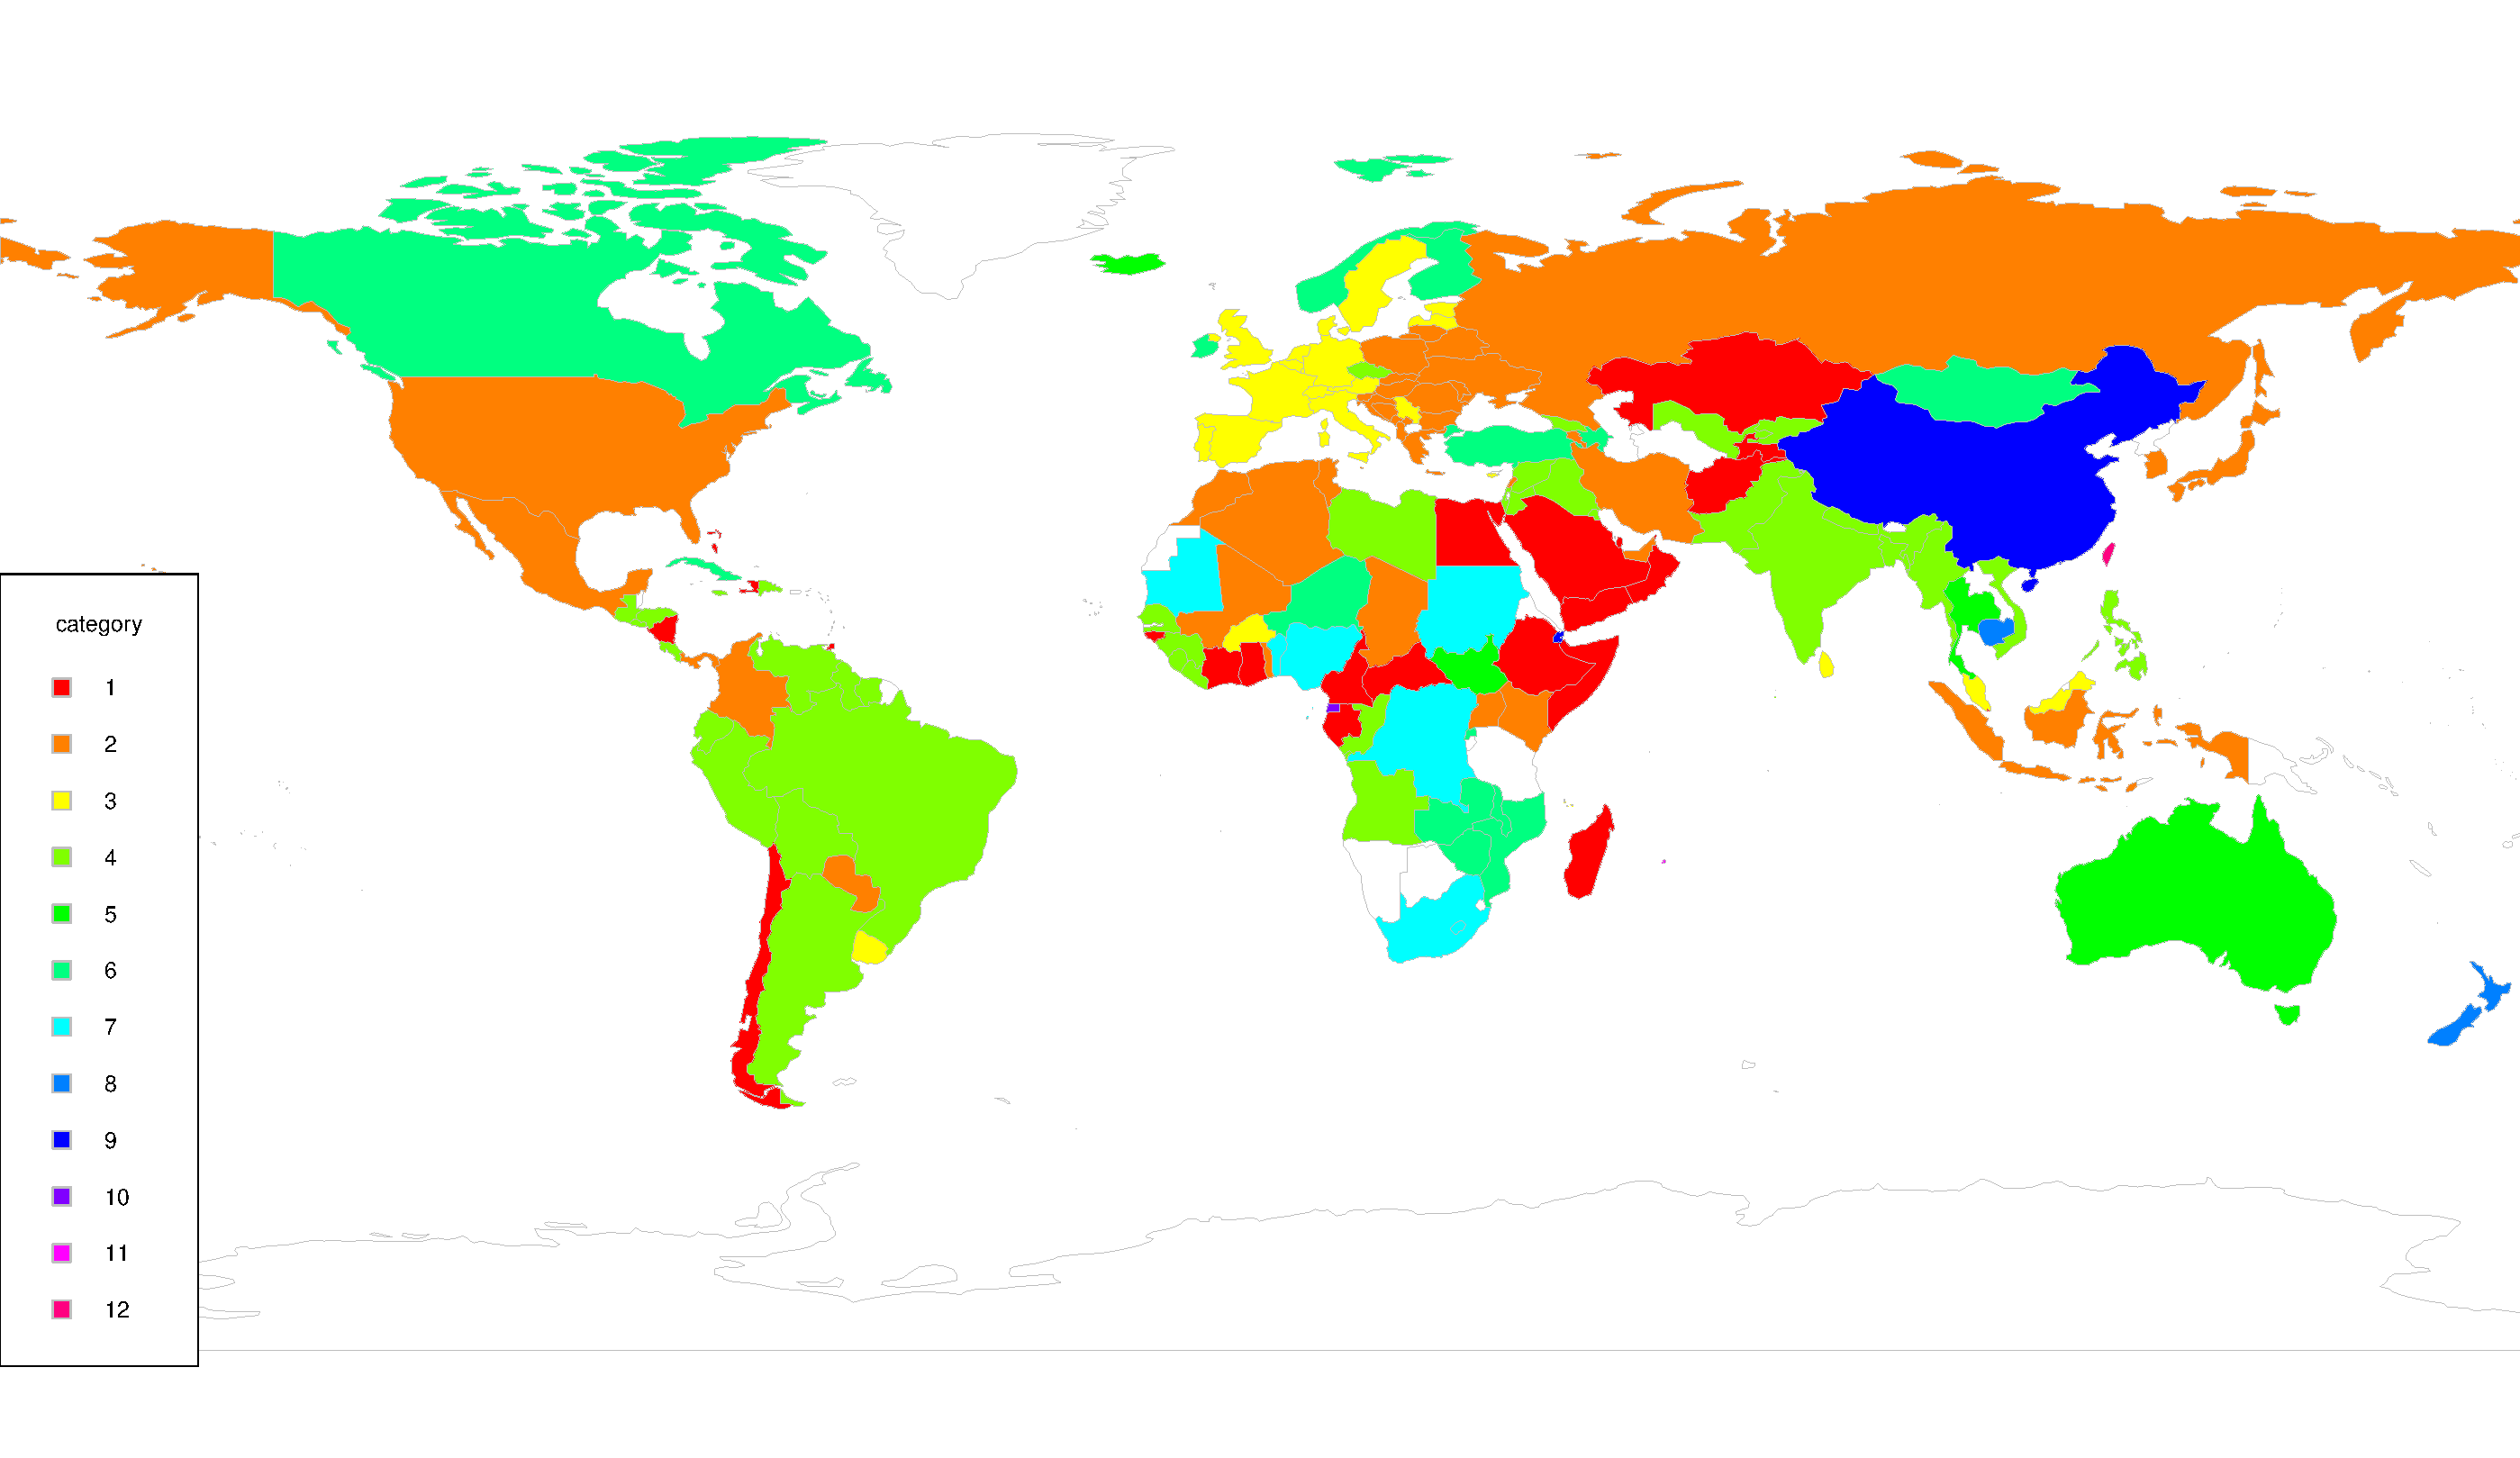
\includegraphics[width=\textwidth]{plots/choropleth_alt_12}
\caption{Results of HAC for $12$ clusters (alternative approach) on a map: each country is coloured according to the group it belongs to.}
\end{minipage}
\end{figure}

\newpage 
\FloatBarrier
\begin{sidewaysfigure}[t!]
%\begin{minipage}[t]{0.98\textwidth}
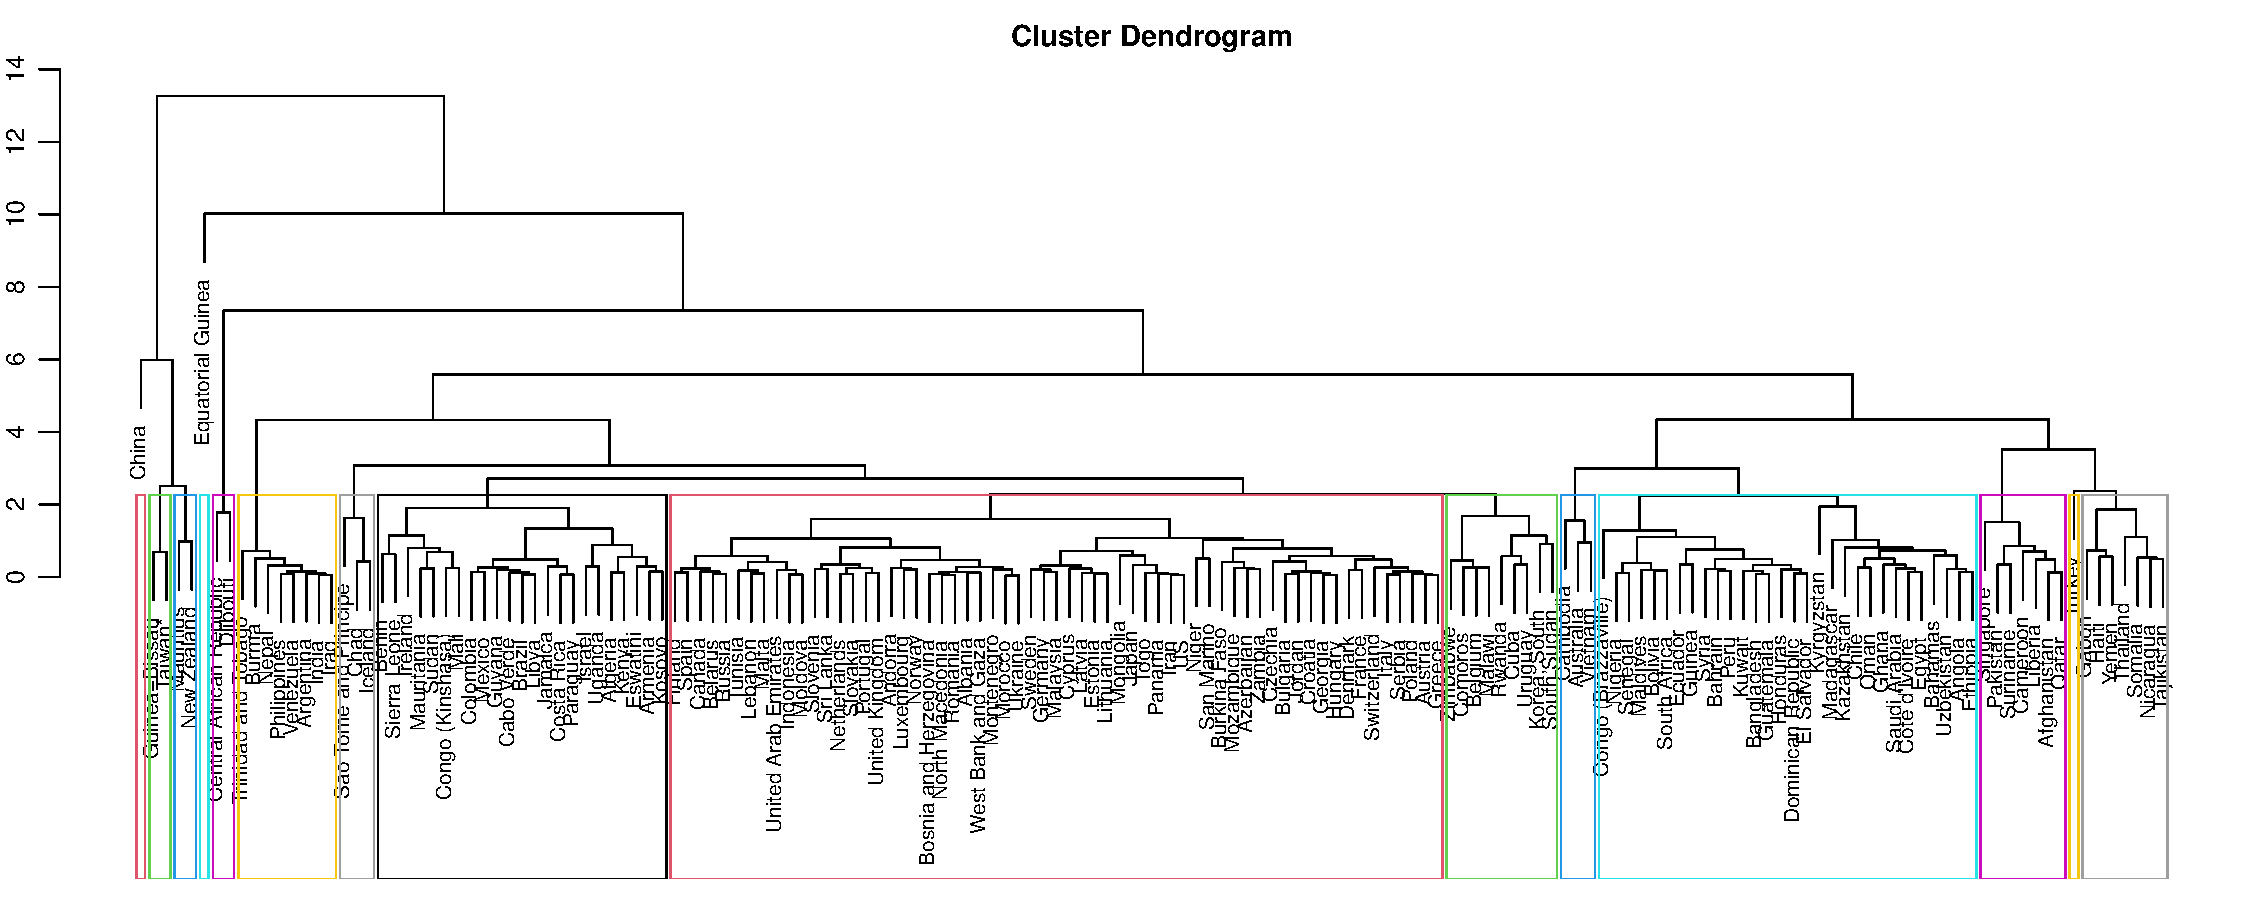
\includegraphics[width=\textwidth]{plots/dendrogram_15}
\caption{Results of HAC for $15$ clusters.}
%\end{minipage}
\end{sidewaysfigure}

\newpage 
\FloatBarrier
\begin{sidewaysfigure}[t!]
%\begin{minipage}[t]{0.98\textwidth}
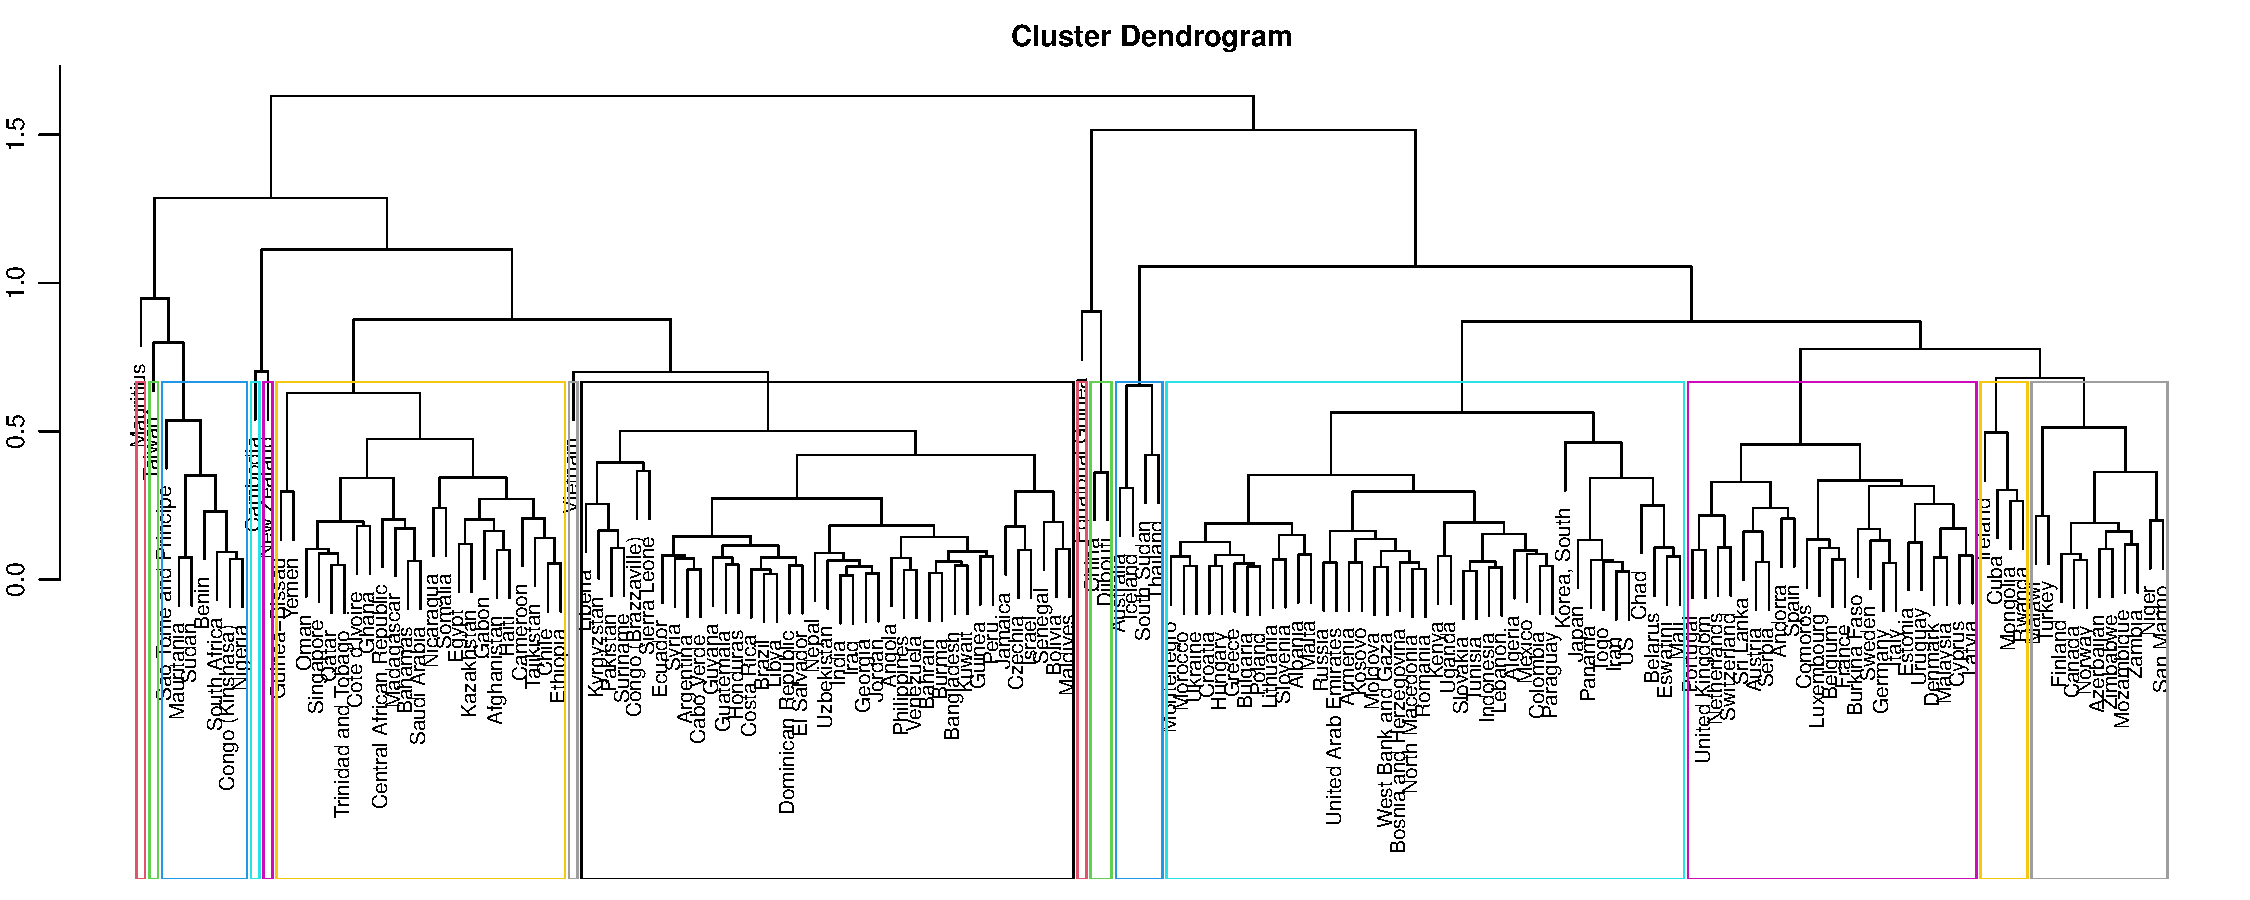
\includegraphics[width=\textwidth]{plots/dendrogram_alt_15}
\caption{Results of HAC for $15$ clusters, alternative approach}
%\end{minipage}
\end{sidewaysfigure}


\begin{figure}[t!]
\begin{minipage}[t]{0.98\textwidth}
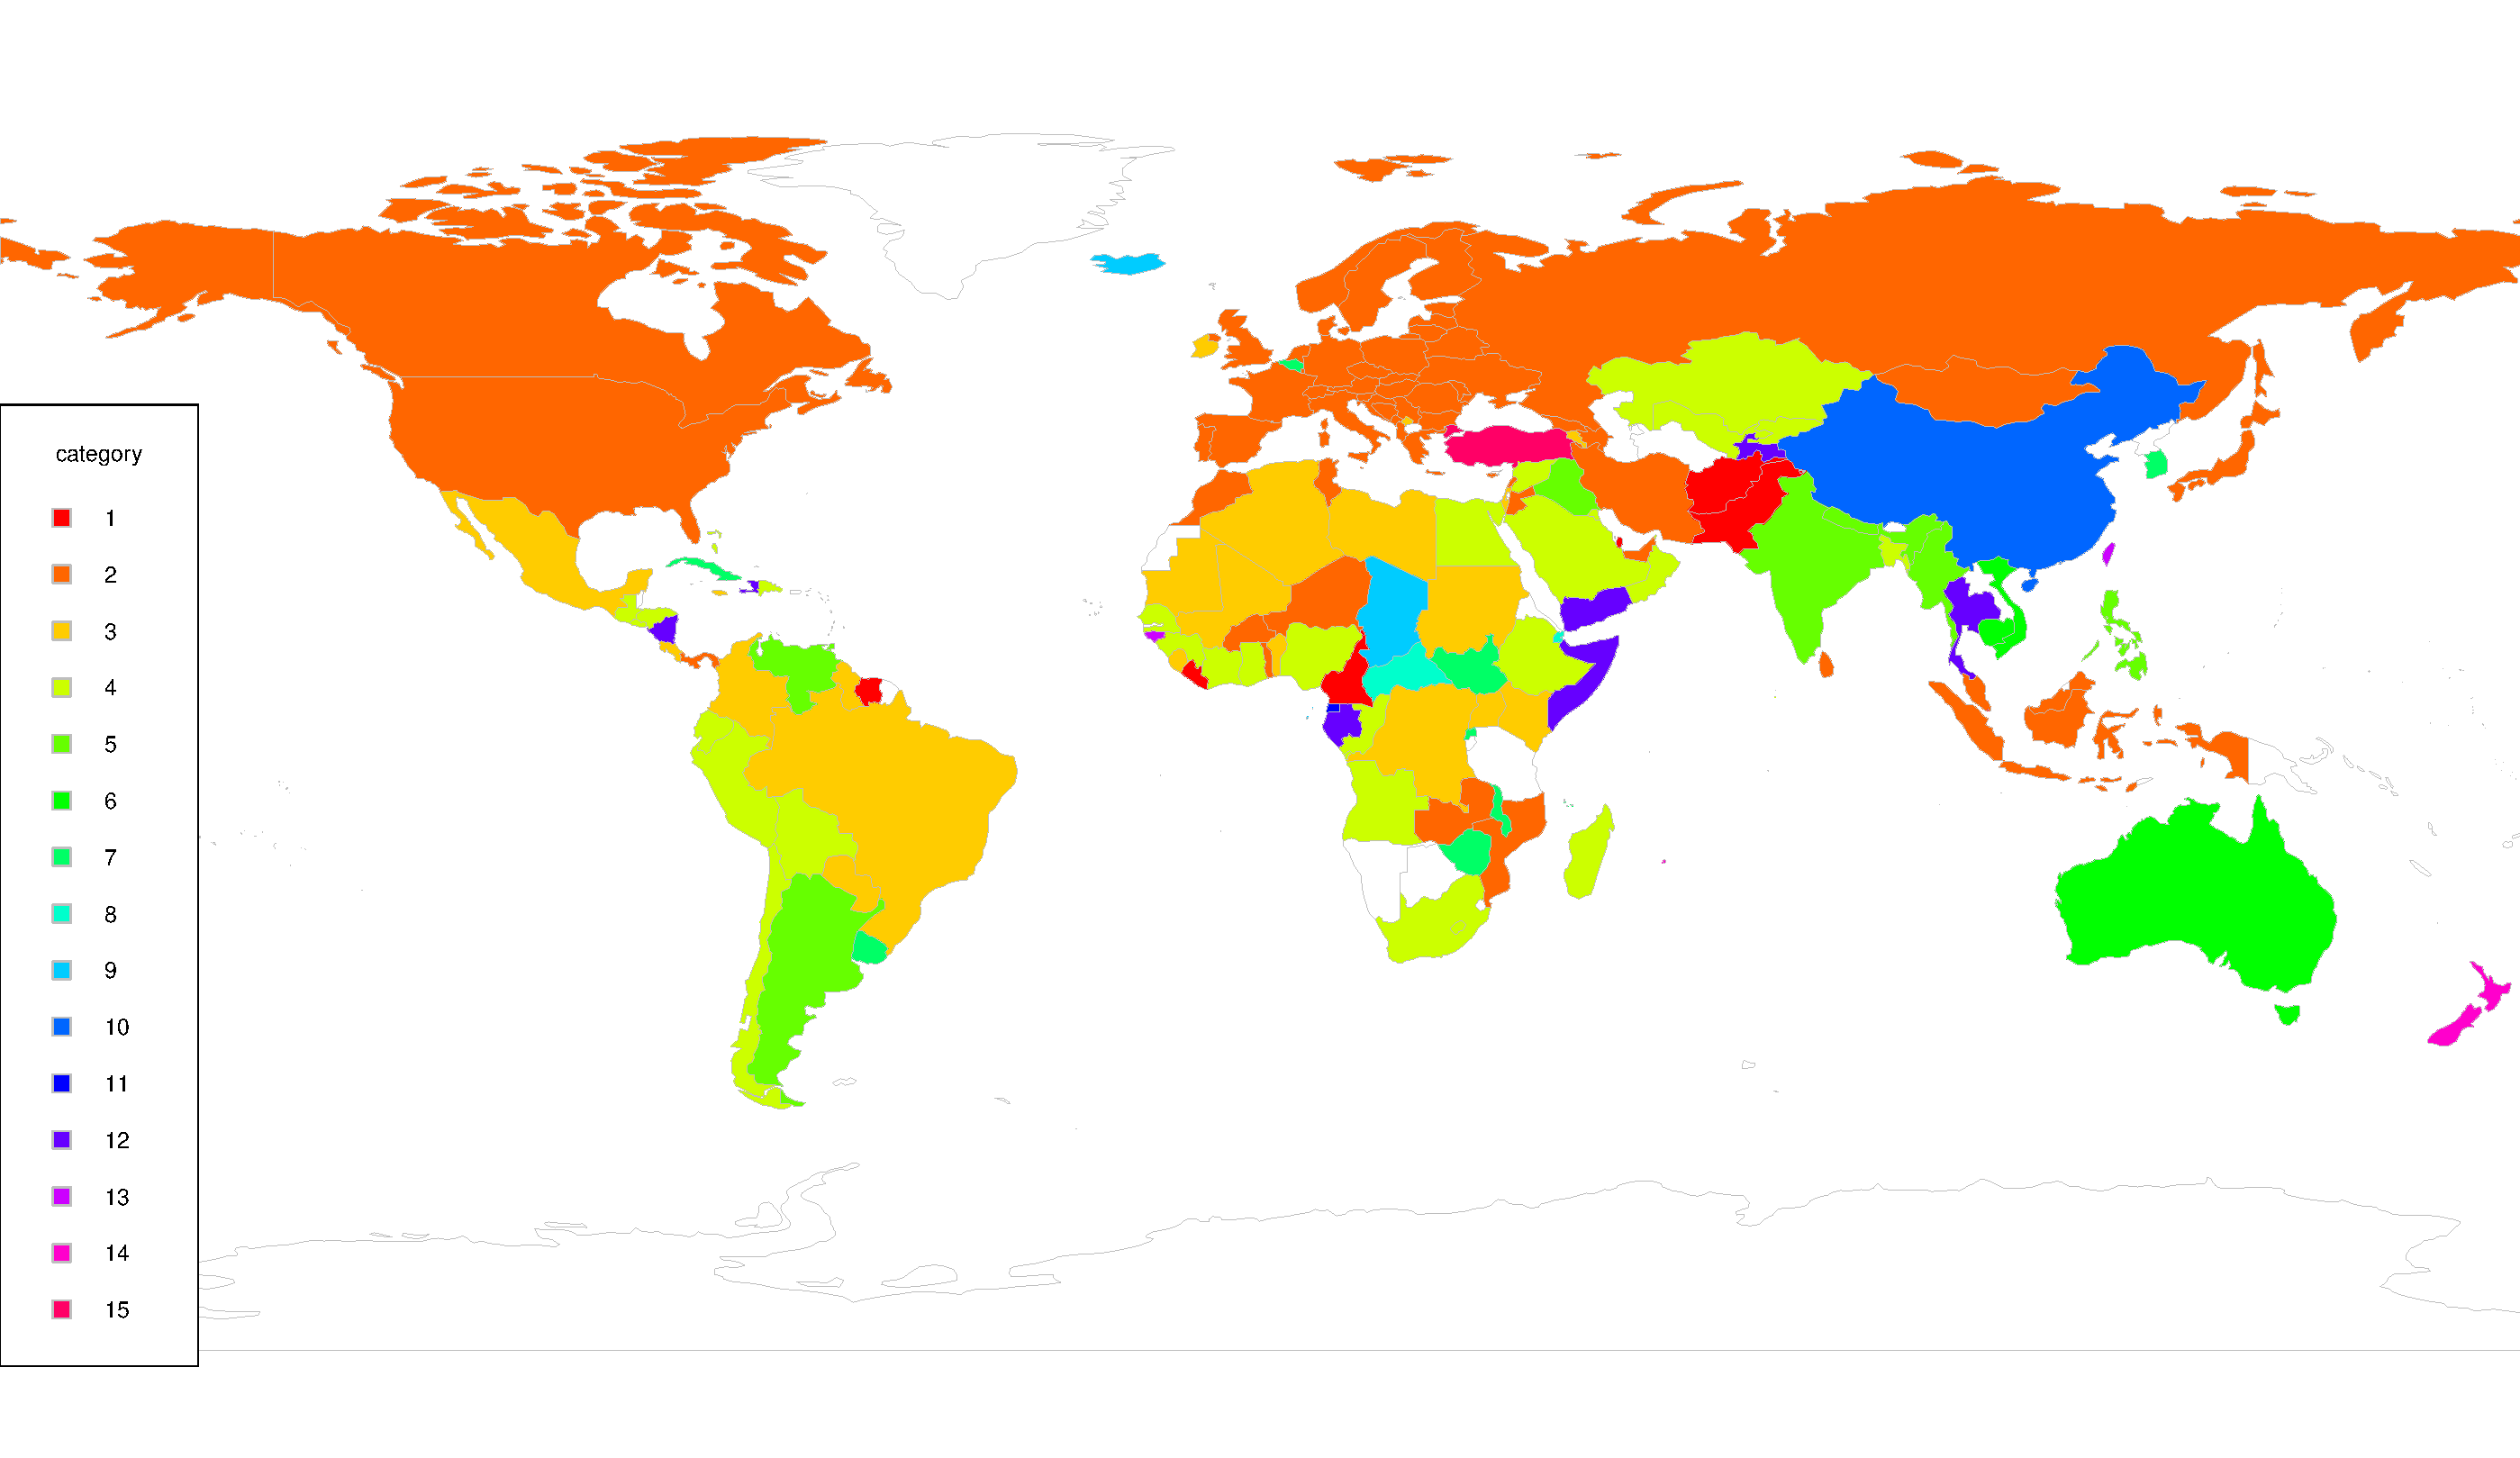
\includegraphics[width=\textwidth]{plots/choropleth_15}
\caption{Results of HAC for $15$ clusters on a map: each country is coloured according to the group it belongs to.}
\end{minipage}
\end{figure}

\begin{figure}[t!]
\begin{minipage}[t]{0.98\textwidth}
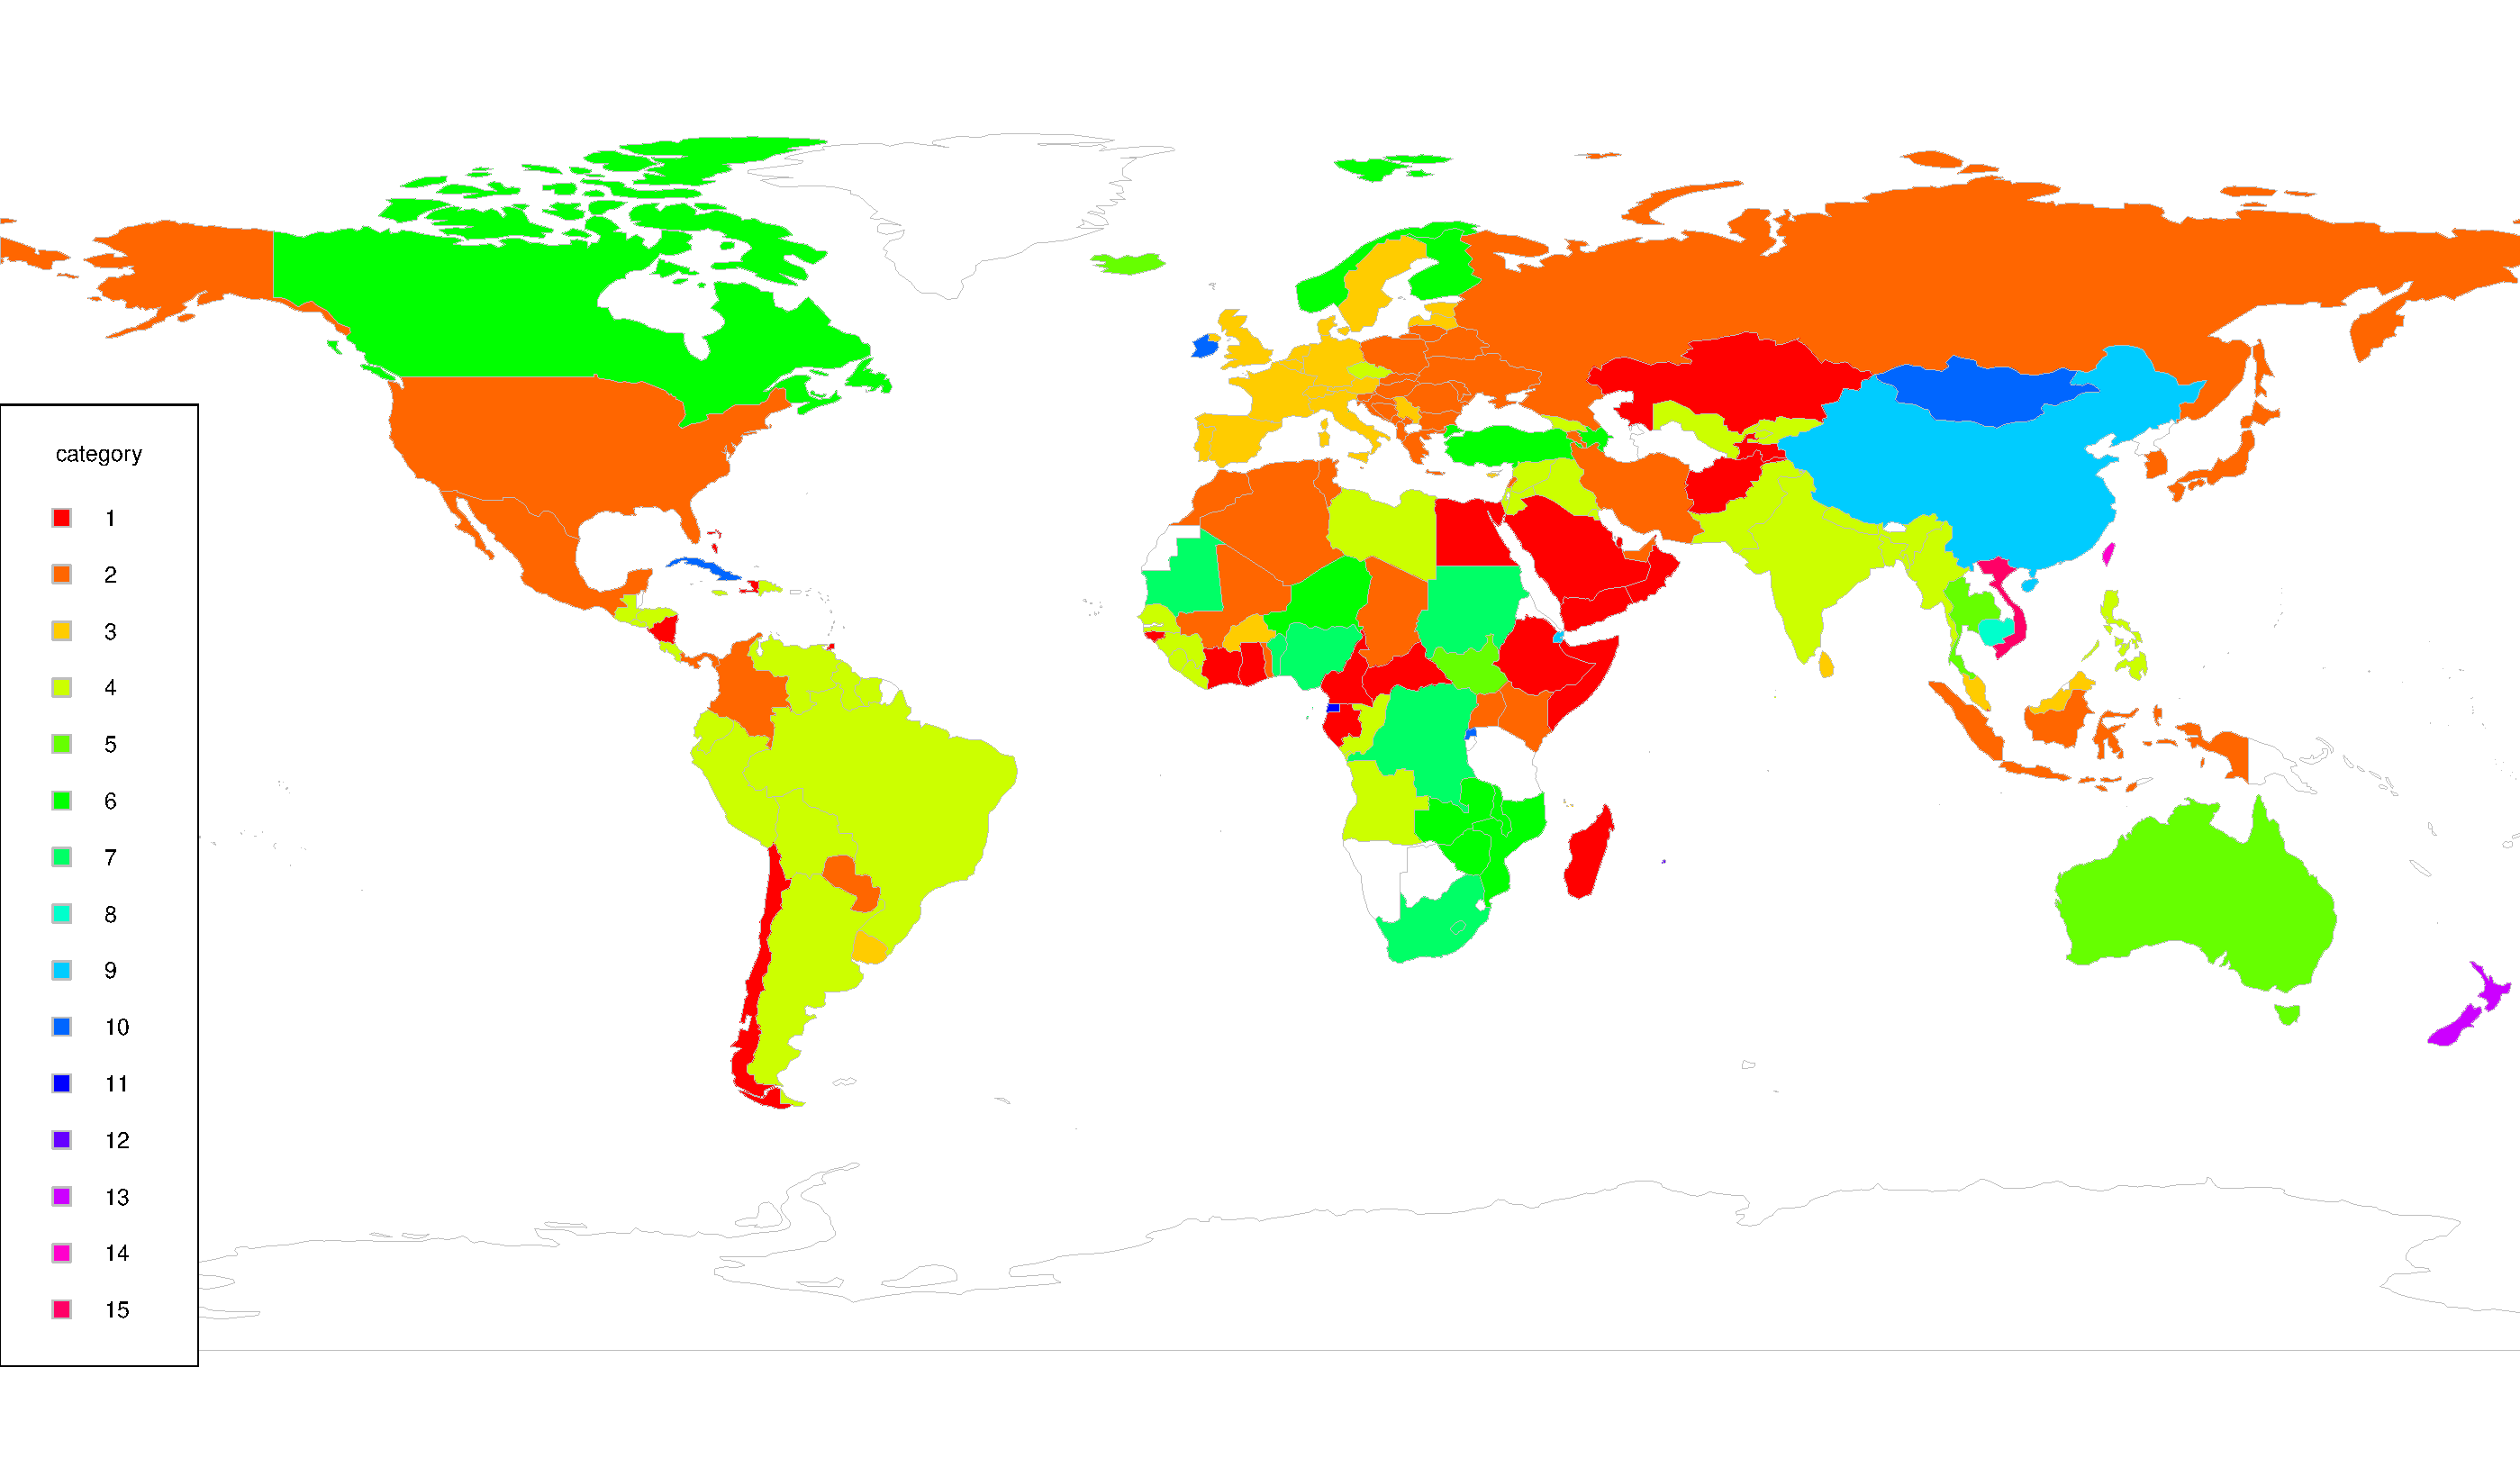
\includegraphics[width=\textwidth]{plots/choropleth_alt_15}
\caption{Results of HAC for $15$ clusters (alternative approach) on a map: each country is coloured according to the group it belongs to.}
\end{minipage}
\end{figure}


%\newpage 
%\FloatBarrier
%\begin{sidewaysfigure}[t!]
%%\begin{minipage}[t]{0.98\textwidth}
%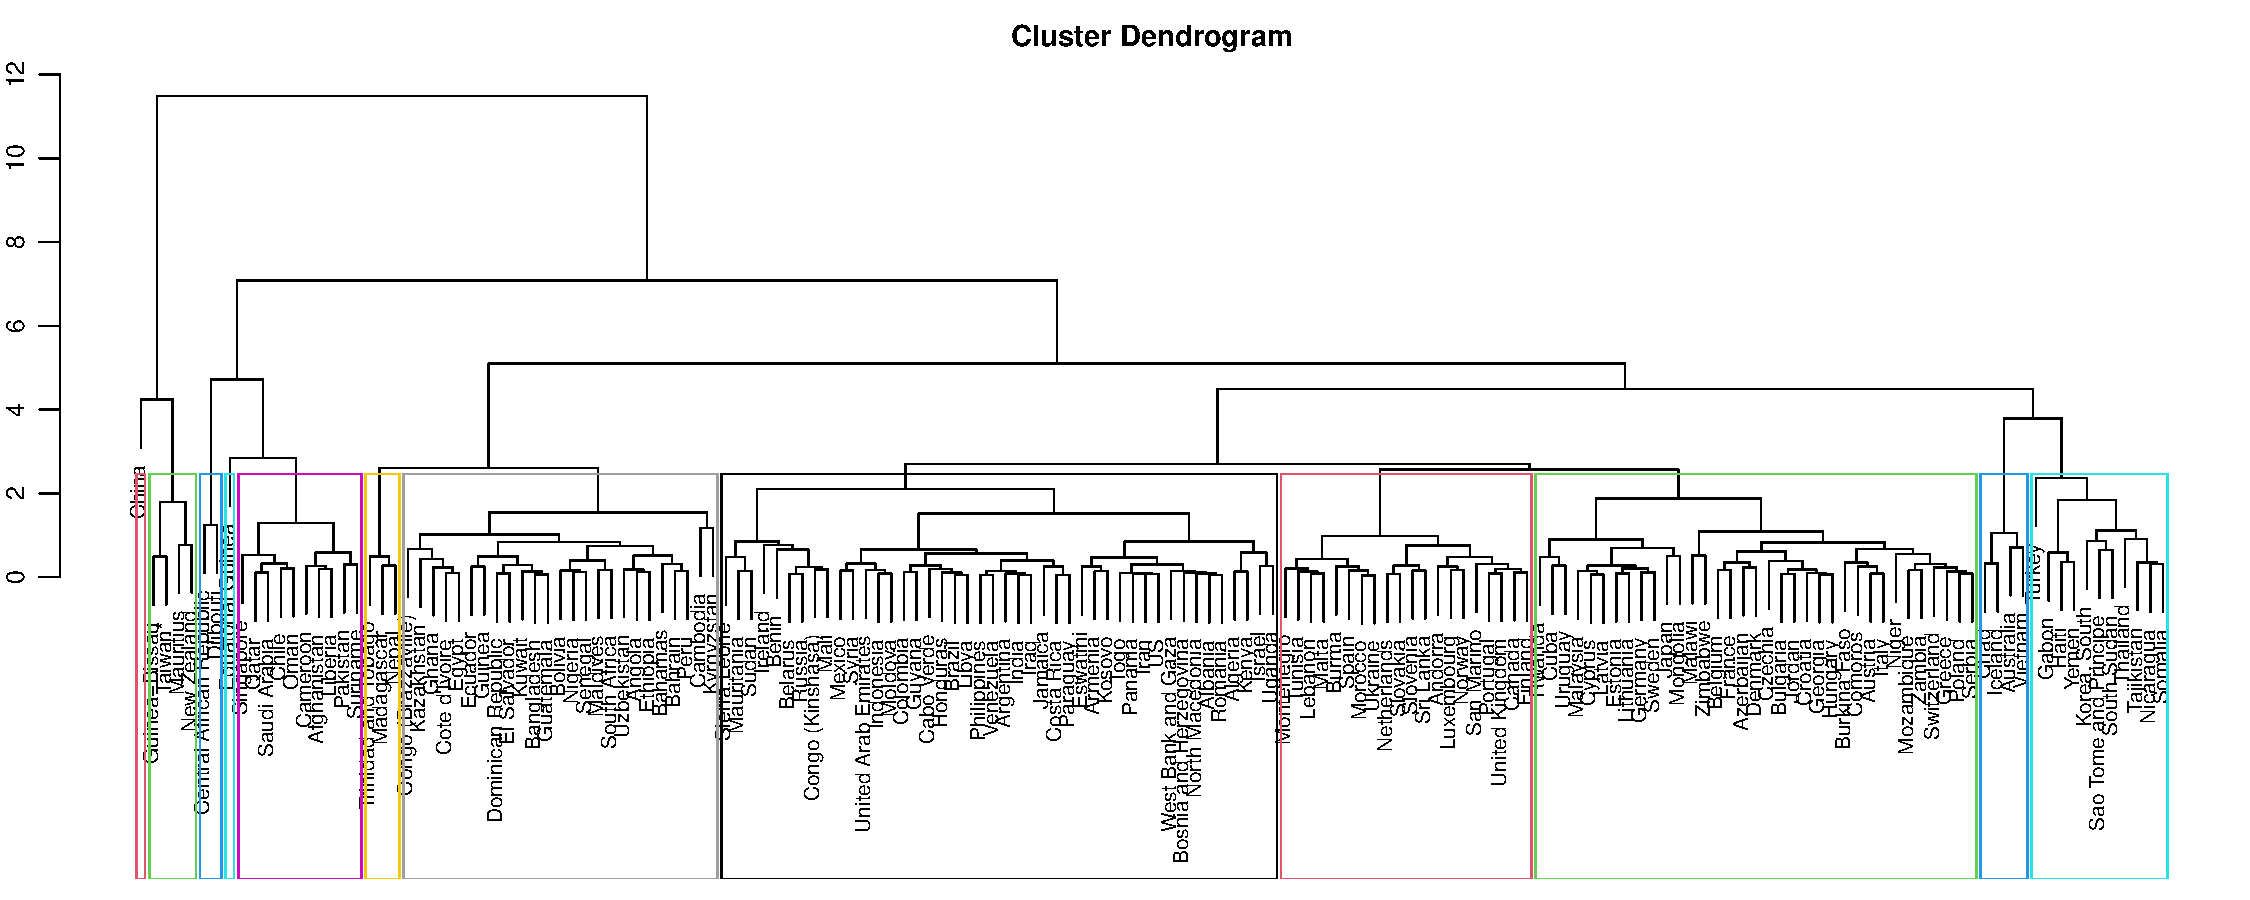
\includegraphics[width=\textwidth]{plots/14days/dendrogram}
%\caption{Results of HAC for $h = 7/T$.}\label{fig:dend_14days}
%%\end{minipage}
%\end{sidewaysfigure}
%
%\begin{figure}[t!]
%\centering
%\begin{subfigure}[b]{0.48\textwidth}
%\subfloat[][]{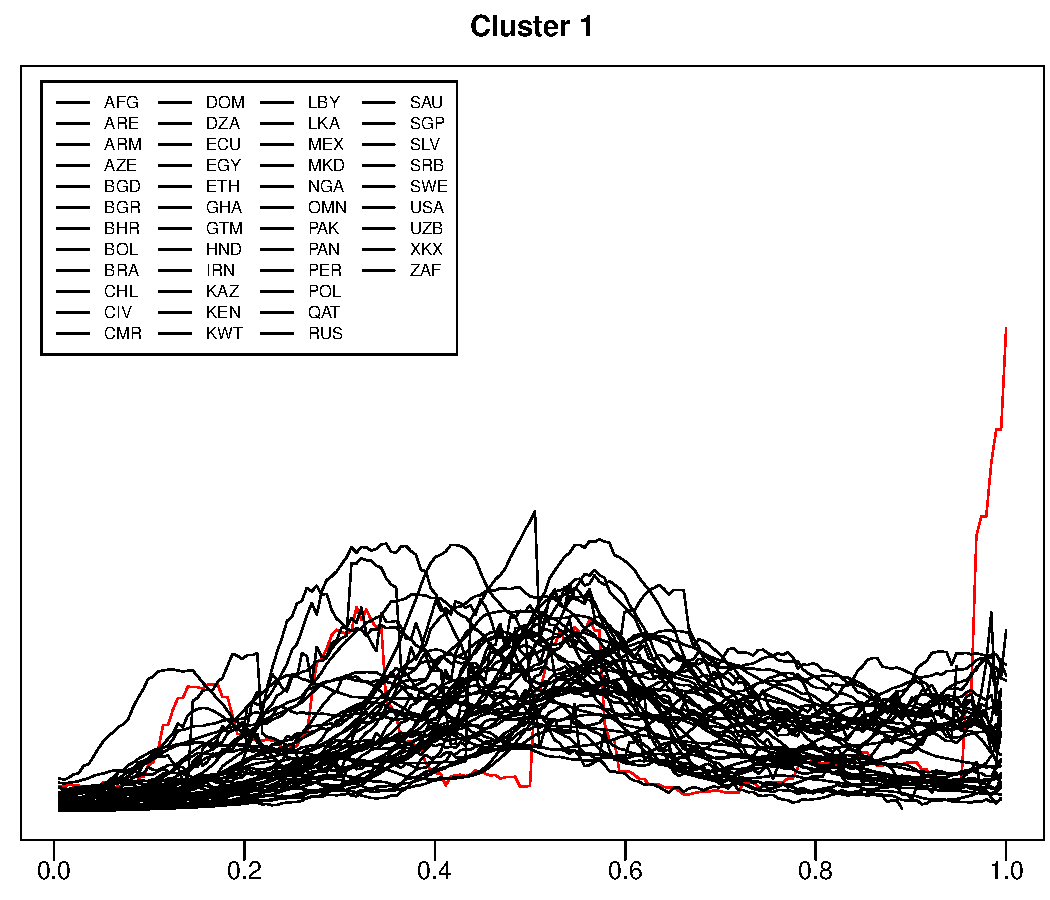
\includegraphics[width=\textwidth]{plots/14days/results_cluster_1}\label{fig:cl1_14days}}
%\end{subfigure}\hspace{0.25cm}
%\begin{subfigure}[b]{0.48\textwidth}
%\subfloat[][]{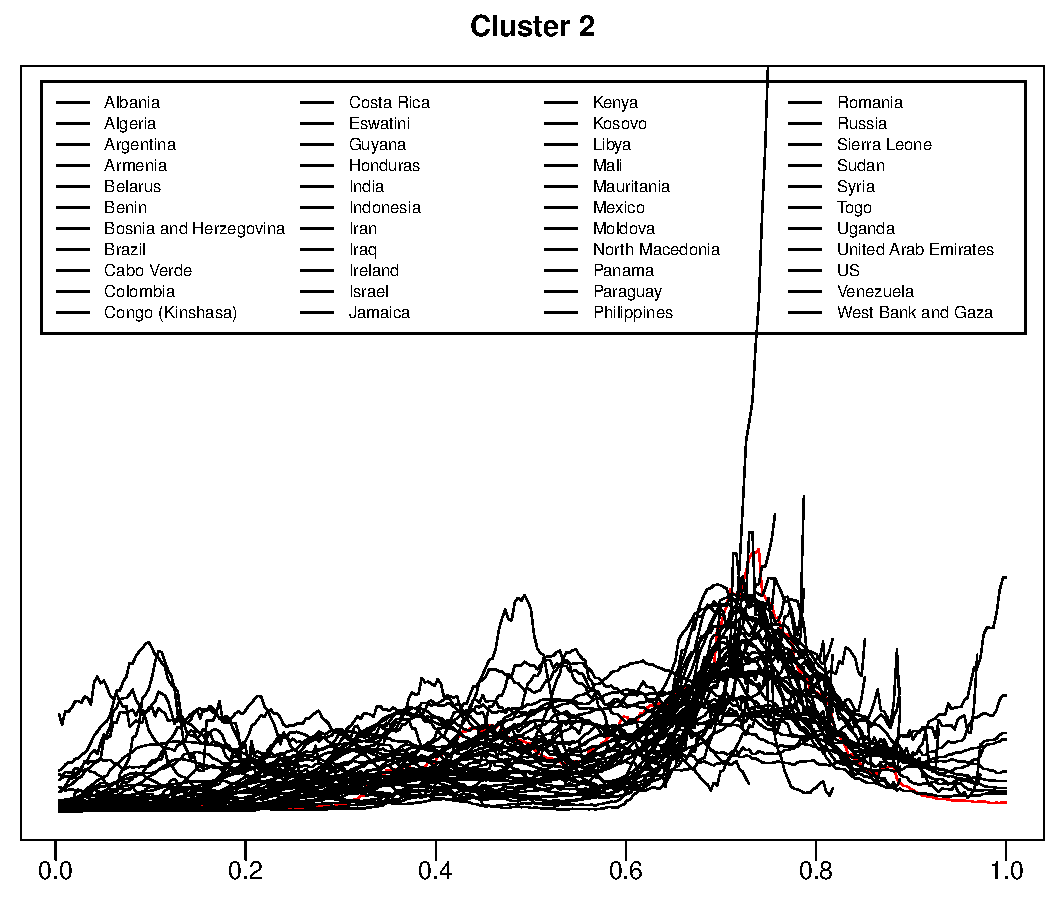
\includegraphics[width=\textwidth]{plots/14days/results_cluster_2}\label{fig:cl2_14days}}
%\end{subfigure}\\
%\begin{subfigure}[b]{0.48\textwidth}
%\subfloat[][]{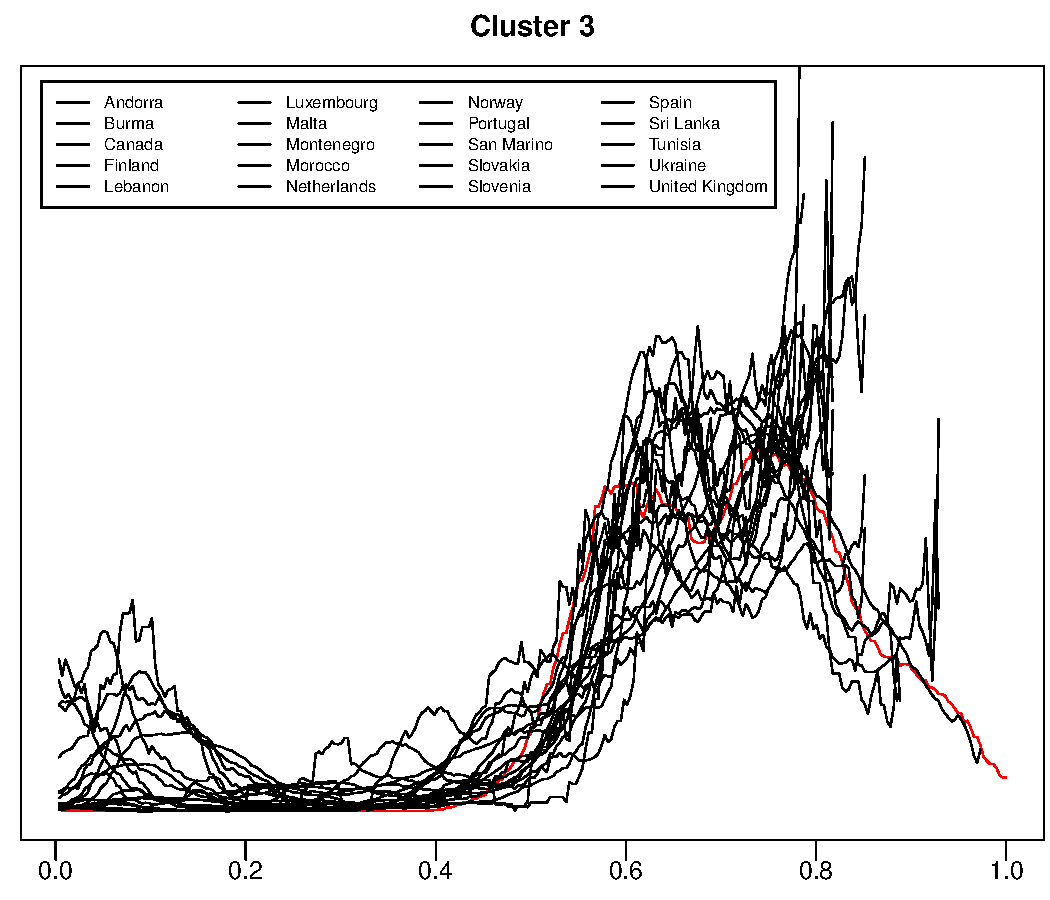
\includegraphics[width=\textwidth]{plots/14days/results_cluster_3}\label{fig:cl3_14days}}
%\end{subfigure}\hspace{0.25cm}
%\begin{subfigure}[b]{0.48\textwidth}
%\subfloat[][]{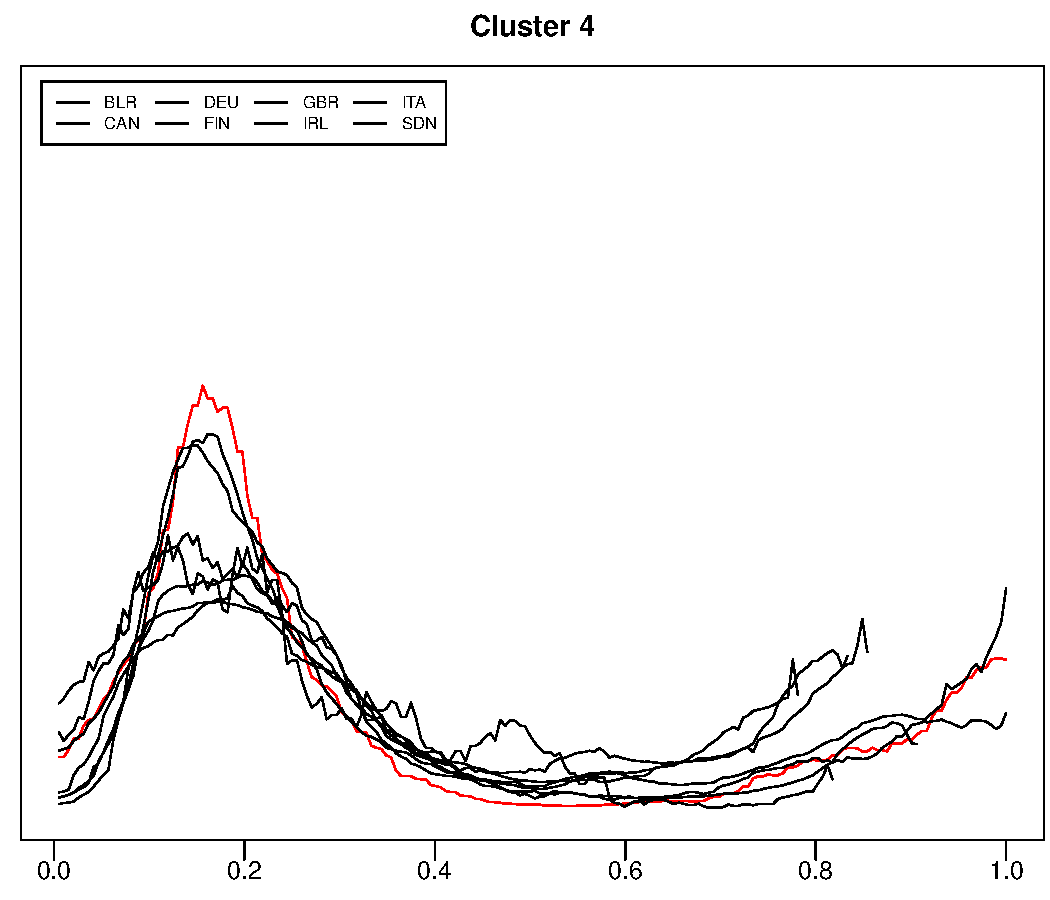
\includegraphics[width=\textwidth]{plots/14days/results_cluster_4}\label{fig:cl4_14days}}
%\end{subfigure}\\
%\begin{subfigure}[b]{0.48\textwidth}
%\subfloat[][]{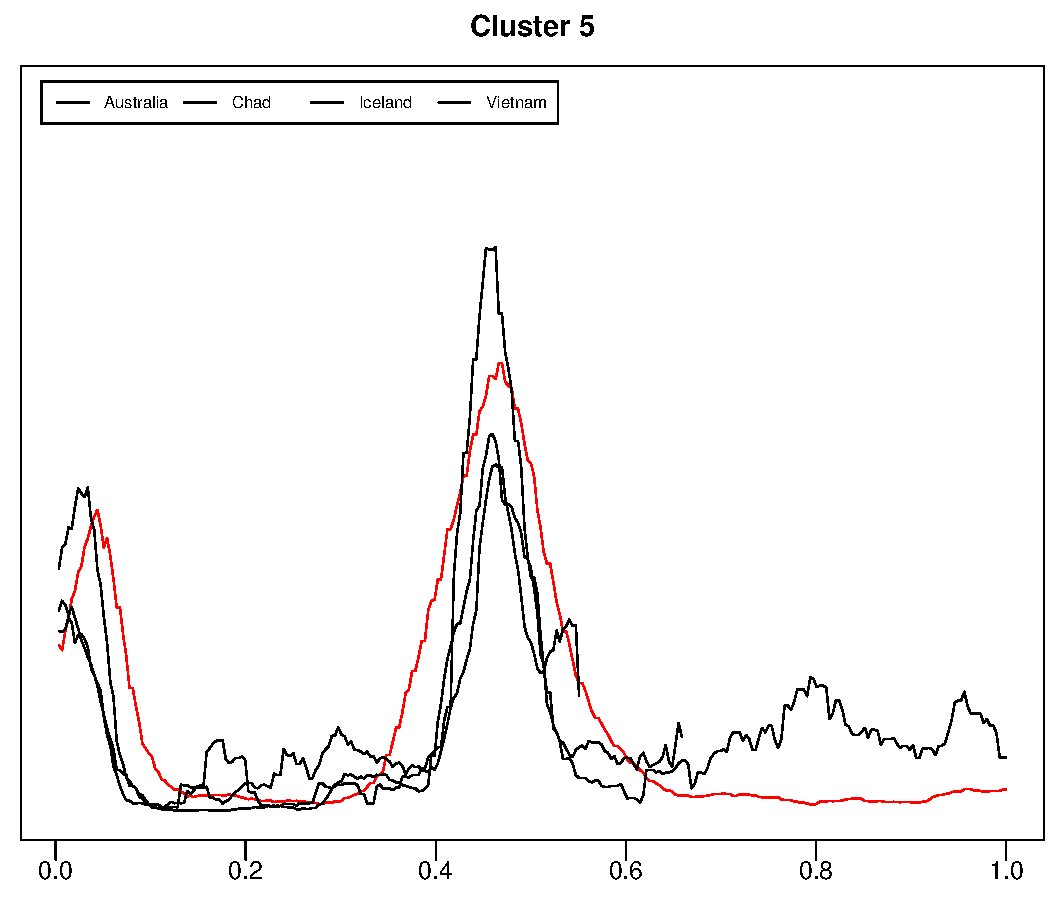
\includegraphics[width=\textwidth]{plots/14days/results_cluster_5}\label{fig:cl5_14days}}
%\end{subfigure}\hspace{0.25cm}
%\begin{subfigure}[b]{0.48\textwidth}
%\subfloat[][]{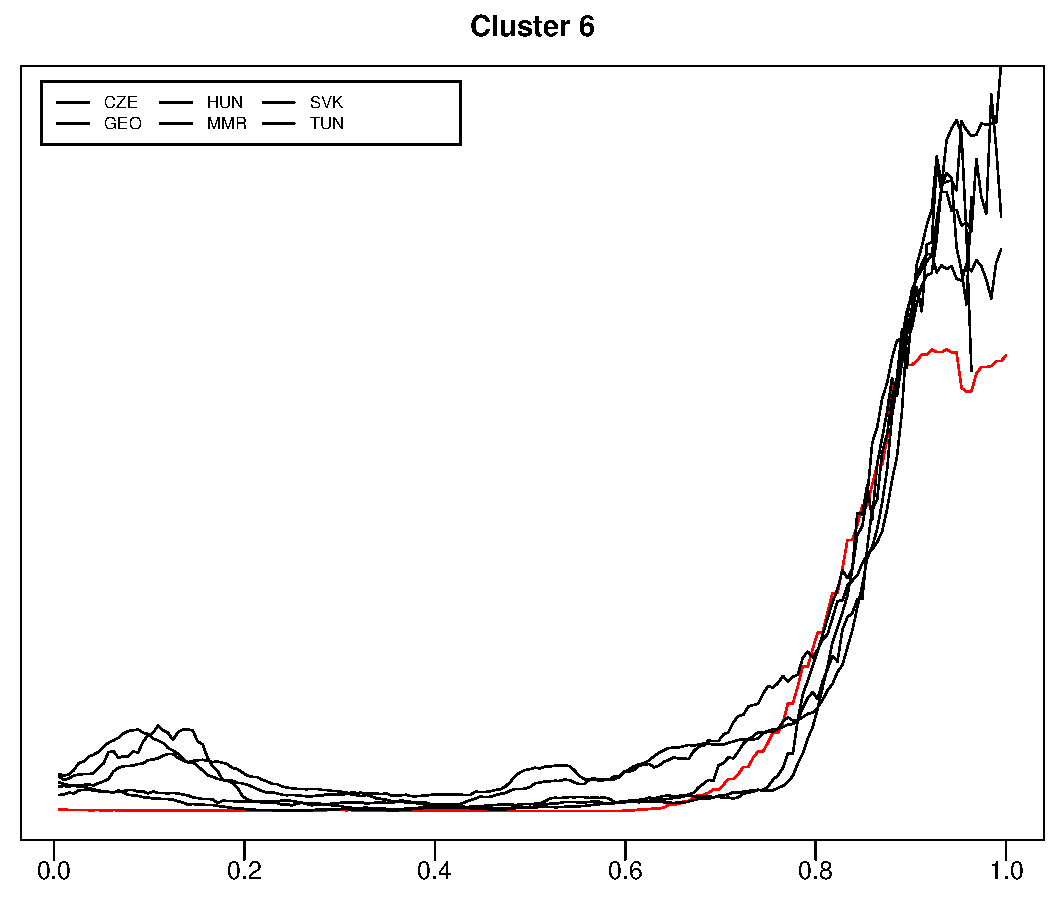
\includegraphics[width=\textwidth]{plots/14days/results_cluster_6}\label{fig:cl6_14days}}
%\end{subfigure}
%\end{figure}
%
%\begin{figure}
%\ContinuedFloat
%\centering
%\begin{subfigure}[b]{0.48\textwidth}
%\subfloat[][]{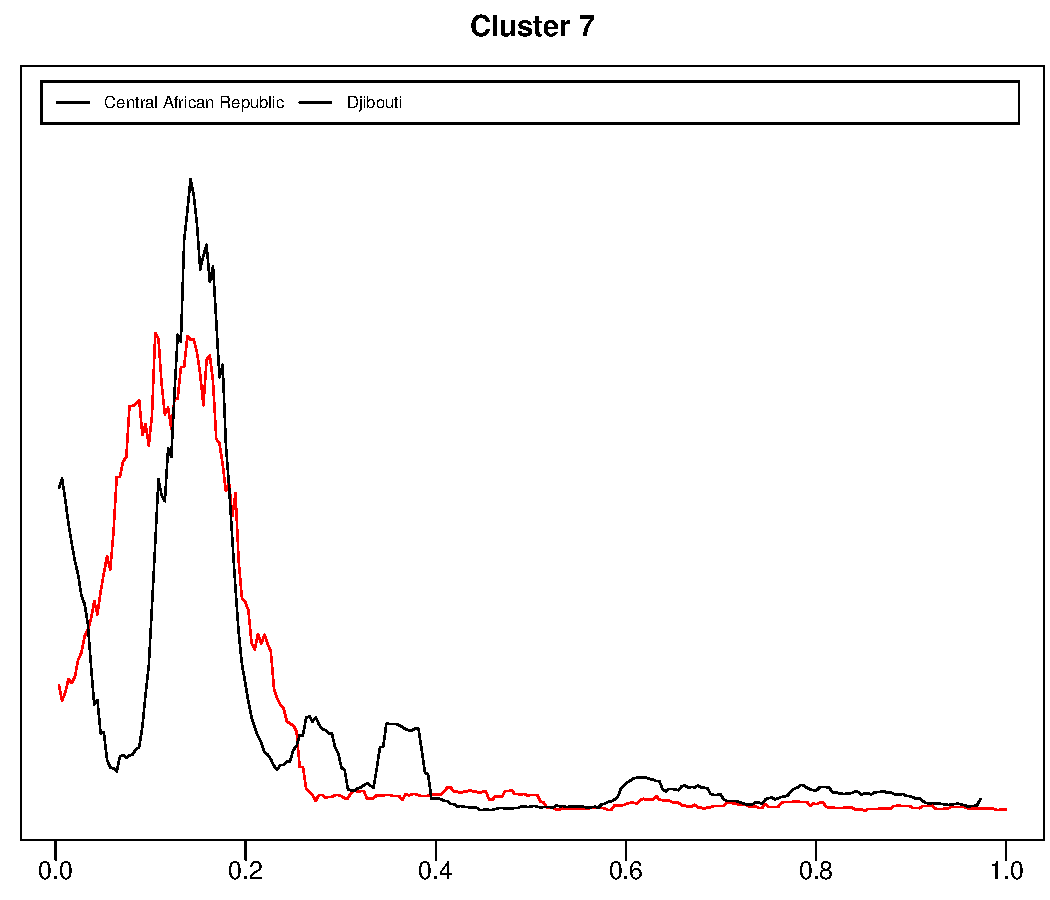
\includegraphics[width=\textwidth]{plots/14days/results_cluster_7}\label{fig:cl7_14days}}
%\end{subfigure}
%\caption{Clusters produced by the algorithm. Each panel presents appropriately scaled curve estimates $\hat{m}_i$ that belong to a particular cluster. The bandwidth $h$ is taken to be $7/T$.}\label{fig:clusters}
%\end{figure}
%
%\begin{figure}[t!]
%\begin{minipage}[t]{0.98\textwidth}
%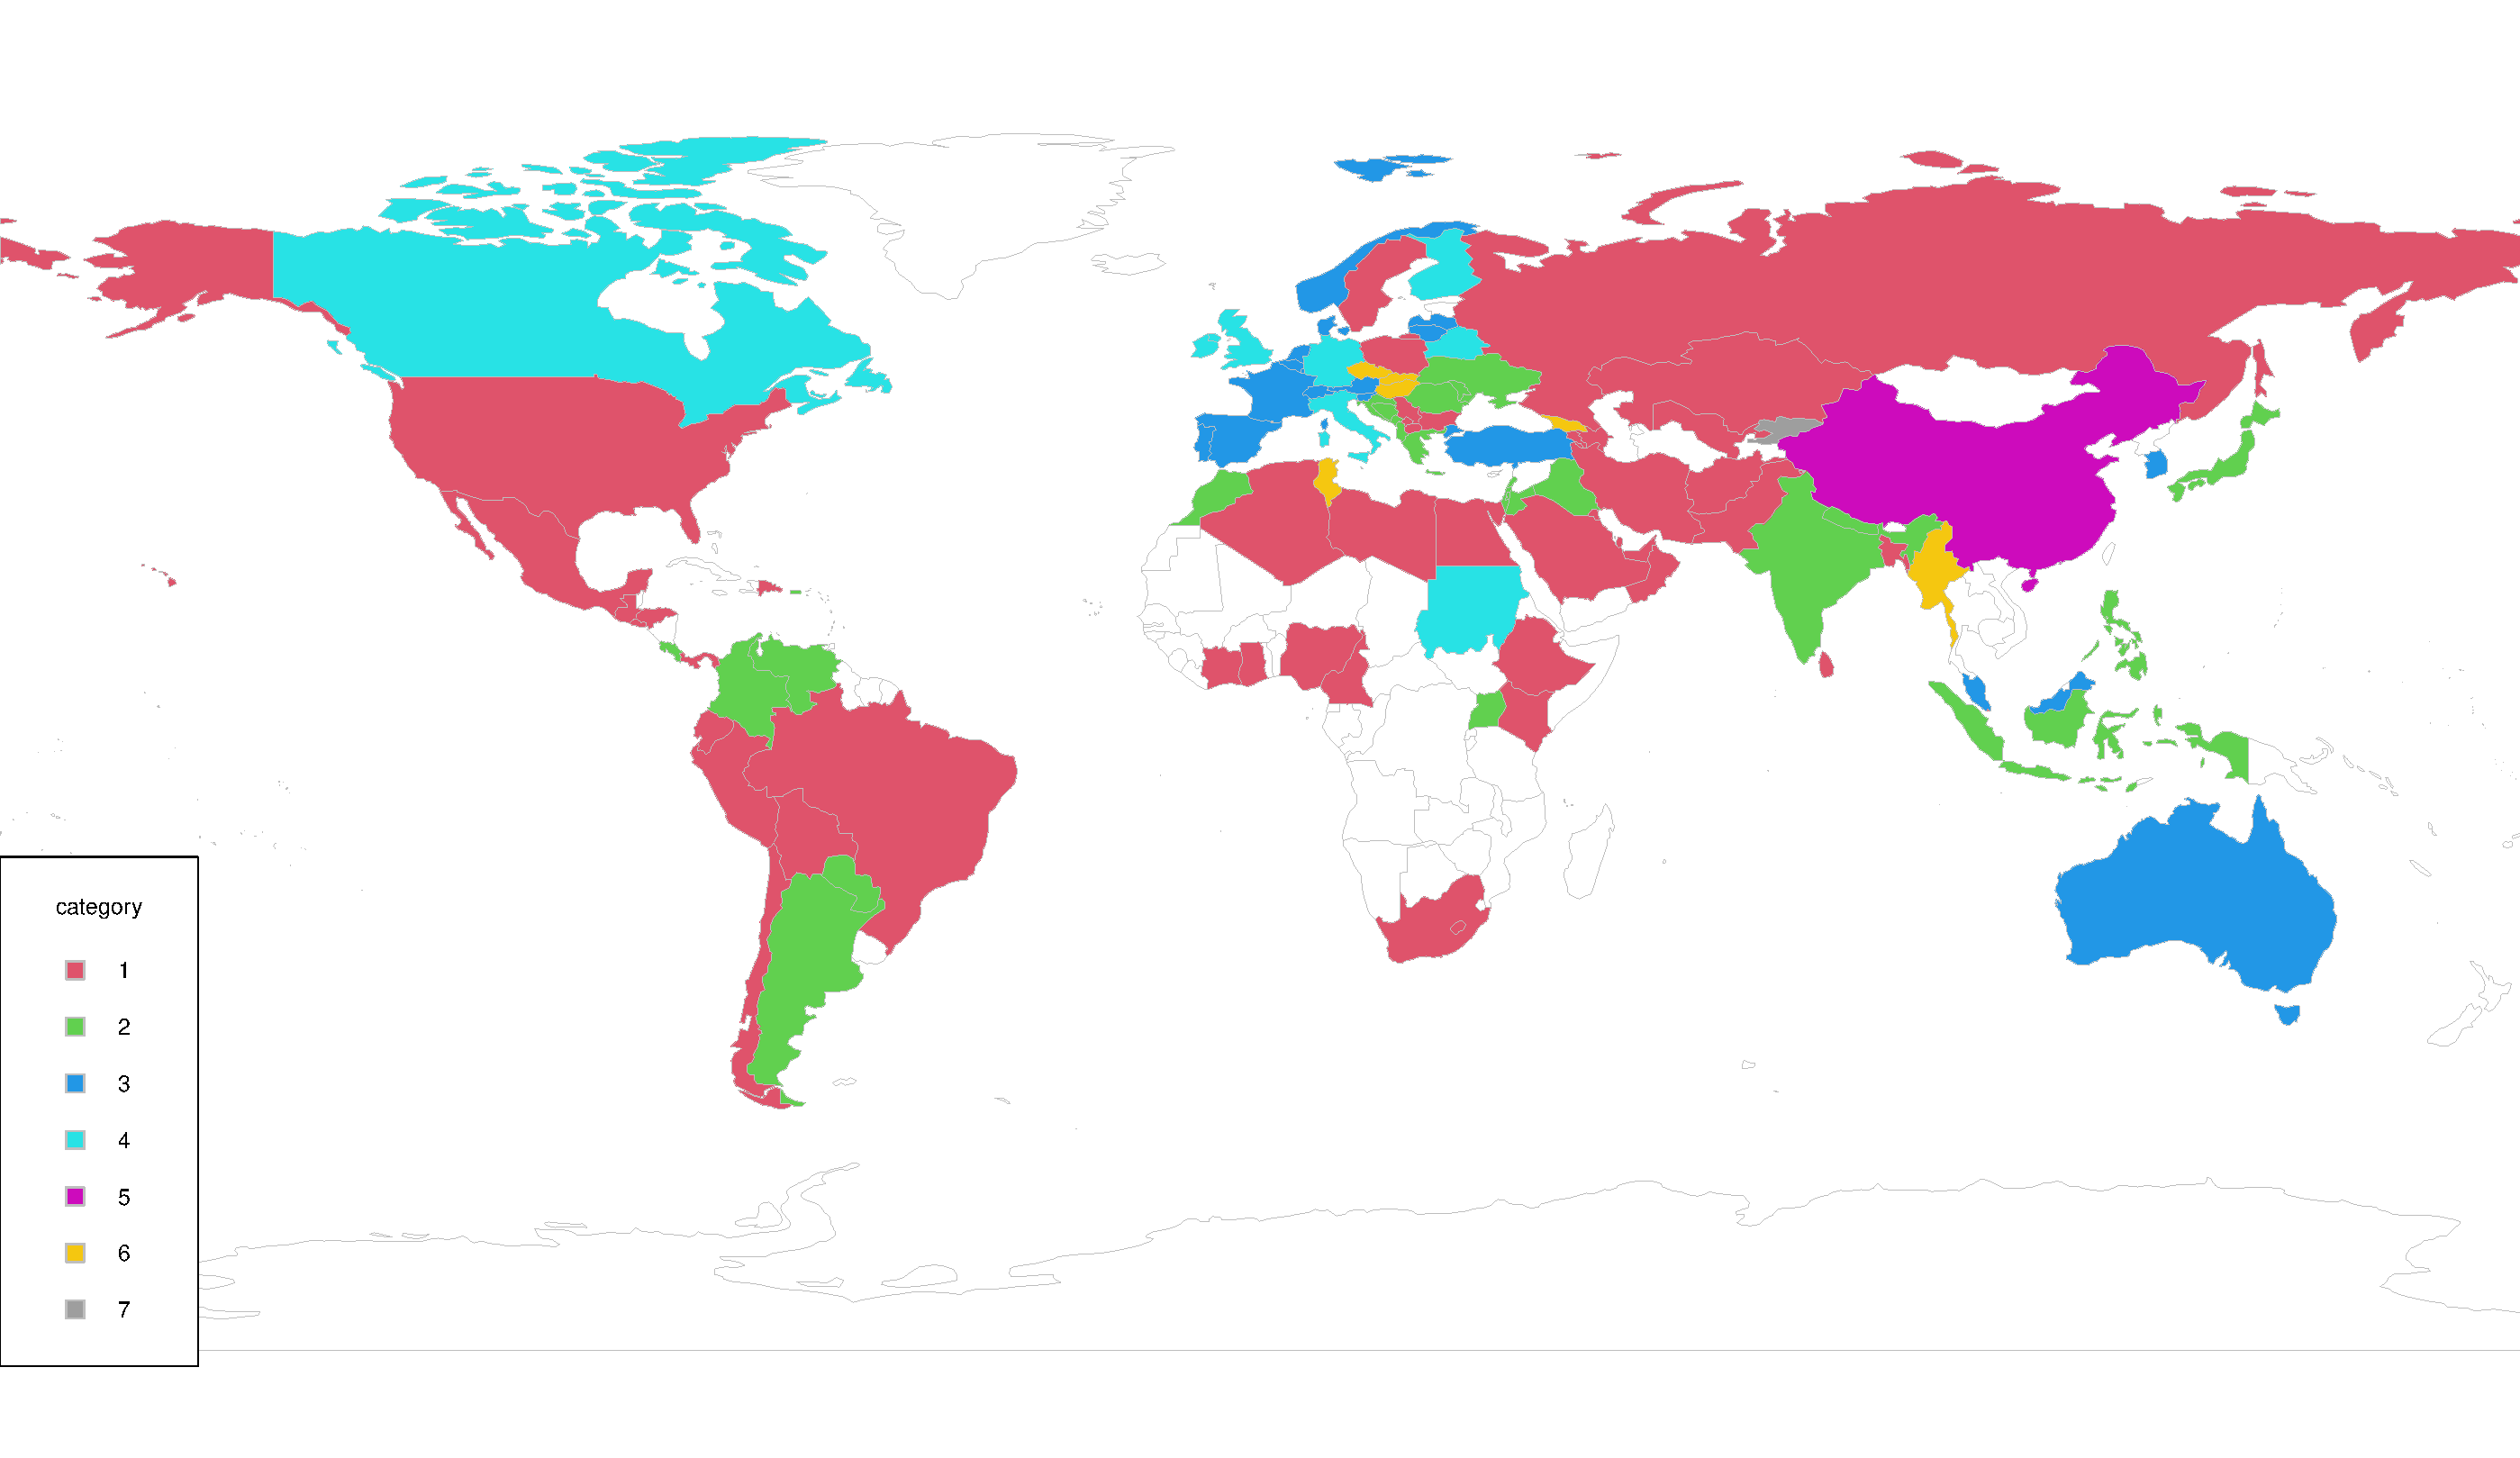
\includegraphics[width=\textwidth]{plots/14days/choropleth}
%\caption{Results of HAC for $h = 7/T$ on a map: each country is coloured according to the group it belongs to.}\label{fig:map_14days}
%\end{minipage}
%\end{figure}



\clearpage
\bibliographystyle{ims}
{\small
\setlength{\bibsep}{0.35em}
\bibliography{bibliography}}



\end{document}
